\documentclass[9pt]{beamer}
\usepackage[utf8]{inputenc}
\usepackage[english]{babel}
\usepackage[T1]{fontenc}
\usepackage{multimedia}
\usepackage[absolute,overlay]{textpos}
\usepackage{graphicx}
\usepackage{tikz}
\usepackage{times}
\usepackage{textcomp}
\usepackage{amsmath}
\usepackage{amssymb}
\usepackage{verbatim}
\usepackage{xcolor}
\usepackage{textpos}
\usepackage{eulervm}
\usepackage{caption}
\usepackage{amsbsy}
\usepackage{feynmp-auto}
\usepackage{hepnicenames}
\usepackage{amsmath}
\usepackage{amssymb}
\usepackage{color}
\usepackage{slashed}
\usepackage{bbold}
\usepackage{array}
\usepackage{color}
\usepackage{colortbl}
\usefonttheme[onlymath]{serif}

\captionsetup{labelformat=empty}

\let\oldmb\mathbold
\protected\def\mathbold{\oldmb}
\usetikzlibrary{arrows,shapes}
\usetikzlibrary{patterns,arrows,decorations.pathreplacing}
\usetheme{Madrid}
\usecolortheme{dolphin}

\newcommand{\nologo}{\setbeamertemplate{logo}{}} % command to set the logo to nothing

%per diagrammi di Feynman
\usepackage[pscoord]{eso-pic}% The zero point of the coordinate systemis the lower left corner of the page (the default).

\newcommand{\placetextbox}[3]{% \placetextbox{<horizontal pos>}{<vertical pos>}{<stuff>}
  \setbox0=\hbox{#3}% Put <stuff> in a box
  \AddToShipoutPictureFG*{% Add <stuff> to current page foreground
    \put(\LenToUnit{#1\paperwidth},\LenToUnit{#2\paperheight}){\vtop{{\null}\makebox[0pt][c]{#3}}}%
  }%
}%
\author[Fabrizio Grosa]%
{
  \footnotesize{\includegraphics[scale=0.35]{logounito.png}\\[3mm] Universit\`{a} degli studi di Torino} - Dipartimento di Fisica \\[5mm] 
  \footnotesize{Candidato: Fabrizio Grosa \\[2mm] Relatore: Prof.ssa Stefania Beolè\\ [2mm] Corelatore: Dott. Francesco Prino \\[2mm] %Controrelatore: Prof. Ernesto Migliore
  }
}
\date{\vspace{-10ex} 20 Febbraio 2016}

\title[Misura dei mesoni $D^+$ prompt]{\huge{Metodi \textit{data-driven} per la misura dei mesoni $D^+$ prompt in collisioni p-Pb a $\sqrt{s_{NN}} = 5.023\text{ }TeV$}}

\begin{document}

{\nologo
\begin{frame}
\maketitle
\end{frame}
}

\section{Heavy Flavours}
\begin{frame}
\frametitle{Perchè studiare gli \textit{heavy flavours}?}
\begin{picture}(320,250)

\put(0,110){\includegraphics[scale=0.23]{ts_cone_hf.png}}

\put(185,255){\captionsetup{labelformat=empty}
\begin{minipage}[t]{0.44\linewidth}
\begin{block}{}
\begin{center}
Gli \textit{heavy flavours} (quark c e b) a causa dell'elevata massa 
\[m_c \simeq 1.5 \text{ }GeV/c^2, \text{ } m_b \simeq 4.5 \text{ } GeV/c^2\]
vengono prodotti nella fase iniziale della collisione (\textit{fase di pre-equilibrio}) 
\[\tau_{prod} \sim \frac{\hslash}{m_{c,b}} \sim 0.1 \text{ }fm/c \]
\end{center}
\end{block}
\end{minipage}}

\put(-5,95){\captionsetup{labelformat=empty}
\begin{minipage}[t]{0.55\linewidth}
\begin{center}
Se nella collisione si crea un mezzo deconfinato (\textit{quark-gluon plasma}), gli heavy flavours interagiscono con esso perdendo energia a causa di scattering elastici con i partoni del mezzo stesso e per radiazione di gluoni (\textit{gluonsstrahlung})
\[\langle \Delta E \rangle \propto \alpha_s C_R \hat{q}L^2\]
\end{center}
\end{minipage}}

\put(230,75){\includegraphics[scale=0.072]{energy_loss.png}}

\put(200,70){\captionsetup{labelformat=empty}
\begin{minipage}[t]{0.4\linewidth}
\begin{center}
La radiazione di gluoni dipende dalla massa del quark, in particolare risulta soppressa per 
\[\theta < \frac{M_q}{E_g} \hspace{2cm}\] 
\end{center}
\end{minipage}}

\put(270,30){\captionsetup{labelformat=empty}
\begin{minipage}[t]{0.4\linewidth}
\textcolor{blue}{DEAD CONE \\EFFECT}
\end{minipage}}

\end{picture} 
\end{frame}

\begin{frame}
\frametitle{\textit{Open heavy flavours} in collisioni p-Pb}
\begin{picture}(320,250)

\put(0,15){\includegraphics[scale=0.35]{PDF_nuclear.png}}
\put(60,125){\includegraphics[scale=0.2]{random_walk.png}}
\put(210,115){\includegraphics[scale=0.25]{cronin_enhancement.png}}

\put(0,230){\captionsetup{labelformat=empty}
\begin{minipage}[t]{1.\linewidth}
\begin{center}
 Nelle collisioni p-A non si raggiungono le condizioni per la formazione del QGP \\
 $\Rightarrow$ ci permettono di studiare gli effetti di \textit{stato iniziale}
 \begin{itemize}
 \color{blue}
  \item Cronin Enhancement
  \vspace{2.8cm}
  \item Modifica delle PDF in presenza di materia nucleare
 \end{itemize}
\end{center}
\end{minipage}}

\put(10,192){\captionsetup{labelformat=empty}
\begin{minipage}[t]{0.55\linewidth}
Le collisioni multiple dei partoni del proiettile con i nucleoni del nucleo determinano uno \textit{shift} dello spettro a più alti valori di momento trasverso $p_T$
\end{minipage}}

\put(145,90){\captionsetup{labelformat=empty}
\begin{minipage}[t]{0.58\linewidth}
Si possono distringuere quattro regioni:
\begin{itemize}
 \item $x \lesssim 0.1$ $\rightarrow F_2^A/F_2^N < 1$ \textit{shadowing effect} 
 \item $0.1 \lesssim x \lesssim 0.2\text{ }\rightarrow$ \textit{anti-shadowing} 
 \item $0.2 \lesssim x \lesssim 0.8\text{ }\rightarrow$ minimo di $F_2^A/F_2^N$ \textit{EMC effect} 
 \item $x \gtrsim 0.8$ $\rightarrow$ aumento a causa del moto di Fermi
\end{itemize}
\end{minipage}}

\end{picture} 
\end{frame}

\section{ALICE}
\begin{frame}
\frametitle{A Large Ion Collider Experiment}
\begin{picture}(320,250)

\put(0,80){\includegraphics[scale=0.055]{2012-Aug-02-ALICE_3D_v0.jpg}}
\put(10,10){\fcolorbox{red}{white}{\includegraphics[scale=0.18]{2012-Aug-02-ALICE_3D_ITS.jpg}}}
\put(225,160){\fcolorbox{green}{white}{\includegraphics[scale=0.5]{TPC.jpeg}}}
\put(235,20){\fcolorbox{blue}{white}{\includegraphics[scale=0.13]{TOF.png}}}

\put(50,80){
\begin{tikzpicture}[->]
\draw[draw=red,solid,line width=0.2mm] (0, 0) -- + (-0.75,-2.8);
\end{tikzpicture}}

\put(95,175){
\begin{tikzpicture}[->]
\draw[draw=green,solid,line width=0.2mm] (0, 0) -- + (4.3,1);
\end{tikzpicture}}

\put(95,80){
\begin{tikzpicture}[->]
\draw[draw=blue,solid,line width=0.2mm] (0, 0) -- + (4.5,-1.8);
\end{tikzpicture}}

\put(80,60){\captionsetup{labelformat=empty}
\begin{minipage}[t]{0.53\linewidth}
 \hspace{0.1cm} \fcolorbox{red}{white}{{Inner Tracking System}}
\small
\begin{itemize}
\item 2 layer Silicon Pixel Detector
 \item 2 layer Silicon Drift Detector
 \item 2 layer Silicon Strip Detector
\end{itemize}
\end{minipage}}

\put(241,105){\captionsetup{labelformat=empty}
\begin{minipage}[t]{0.53\linewidth}
 \hspace{0.1cm} \fcolorbox{blue}{white}{{Time of Flight}}
\end{minipage}}

\put(230,145){\captionsetup{labelformat=empty}
\begin{minipage}[t]{0.53\linewidth}
 \hspace{0.1cm} \fcolorbox{green}{white}{{Time Projection Chamber}}
\end{minipage}}

\end{picture} 
\end{frame}


\begin{frame}
\frametitle{Ricostruzione e selezione di mesoni $D^+$ in ALICE}
\begin{picture}(320,250)

\put(180,80){\includegraphics[scale=0.23]{Dplustokpipi.png}}
\put(5,20){\includegraphics[scale=0.08]{2013-Mar-06-betap_v5.png}}

\put(0,230){\captionsetup{labelformat=empty}
\begin{minipage}[t]{1.\linewidth}
Per questa analisi i mesoni $D^+$ sono ricostruiti nel canale di decadimento 
\end{minipage}}

\put(85,230){\captionsetup{labelformat=empty}
\begin{minipage}[t]{0.5\linewidth}
\begin{block}{}
 \setlength\abovedisplayskip{0pt}
\[D^+\rightarrow K^-\pi^+\pi^+ (BR = 9.13\%)\] 
\end{block}
\end{minipage}}

\put(200,95){\captionsetup{labelformat=empty}
\begin{minipage}[t]{0.5\linewidth}
$c\tau = 312\text{ } \mu m$
\end{minipage}}

\put(0,190){\captionsetup{labelformat=empty}
\begin{minipage}[t]{1.\linewidth}
\begin{itemize}
 \item Il segnale è estratto con un'\textcolor{blue}{analisi di massa invariante}
 \vspace{0.2cm}
 \item Vengono applicate selezioni topologiche \\sulle quantità ricostruite per \\ridurre il fondo combinatoriale
\end{itemize}
\end{minipage}}

\put(160,70){\captionsetup{labelformat=empty}
\begin{minipage}[t]{0.53\linewidth}
\begin{itemize}
 \item Per rimuovere ulteriormente del fondo viene applicata la \textit{Particle Identification} (PID) nella selezione delle tracce nello stato finale 
\end{itemize}
\end{minipage}}

\end{picture} 
\end{frame}

\section{Metodi theory-driven per la misura della frazione di $D^+$ prompt}
\begin{frame}
\frametitle{$D^+$ prompt e feed-down}
\begin{picture}(320,250)

\put(15,25){\includegraphics[scale=0.16]{Prompt_sketch2.png}}
\put(185,20){\includegraphics[scale=0.16]{FD_sketch2.png}}

\put(0,230){\captionsetup{labelformat=empty}
\begin{minipage}[t]{1.\linewidth}
Per la misura dei mesoni $D^+$ che sono originati da un quark \textit{charm} prodotto nella \\collisione è necessario separare il contributo di $D^+$ prompt dal segnale totale
\end{minipage}}

\put(15,205){\captionsetup{labelformat=empty}
\begin{minipage}[t]{0.4\linewidth}
\begin{block}{\centering $D^+$ prompt}
\begin{center}
 Derivano direttamente dall'adronizzazione di un quark $c$ \\
 $c \rightarrow D^+$
\end{center}
\end{block}
\end{minipage}}

\put(190,205){\captionsetup{labelformat=empty}
\begin{minipage}[t]{0.4\linewidth}
\begin{block}{\centering $D^+$ feed-down}
\begin{center}
 Derivano dal decadimento di un mesone B \\
 $b \rightarrow B \rightarrow D^++X$
\end{center} 
\end{block}
\end{minipage}}

\end{picture} 
\end{frame}

\begin{frame}
\frametitle{Metodi \textit{theory-driven} per la misura della frazione di $D^+$ prompt}
\begin{picture}(320,250)

\put(0,235){\captionsetup{labelformat=empty}
\begin{minipage}[t]{1.\linewidth}
La frazione di $D^+$ prompt può essere ottenuta utilizzando metodi \textit{theory-driven}
\vspace{0.2cm}
\begin{itemize}
 \item Metodo $N_b$ 
 \[f_{prompt} = 1-\langle T_{pA} \rangle \textcolor{blue}{\bigg{(}\frac{d\sigma}{dp_Tdy}\bigg{)}_{FONLL}^{feeddown}R_{pA}^{feeddown}(p_T)}\frac{(Acc\times \epsilon)_{feeddown}\Delta y \Delta p_T \cdot BR \cdot N_{ev}}{N_{raw}^{D^+}/2}\]
  \item Metodo $f_c$
 \vspace{-0.2cm}
 \[f_{prompt} = \bigg{(} 1+\frac{\textcolor{blue}{\frac{d\sigma}{dp_Tdy}_{FONLL}^{feeddown}}(Acc\times \epsilon)_{feeddown}\textcolor{blue}{R_{pA}^{feeddown}(p_T)}}{\textcolor{blue}{\frac{d\sigma}{dp_Tdy}_{FONLL}^{prompt}}(Acc\times \epsilon)_{prompt}R_{pA}^{prompt}(p_T)}\bigg{)}^{-1}\]
\end{itemize}
\end{minipage}}

\put(0,105){\captionsetup{labelformat=empty}
\begin{minipage}[t]{0.95\linewidth}
\begin{center}
Il calcolo perturbativo di $\textcolor{blue}{d\sigma/dp_Tdy}$ e l'assunzione di \textcolor{blue}{$R_{pA}^{feeddown}(p_T)$} (non è mai stato misurato) comportano un'incertezza, che è uno dei principali contributi all'errore sistematico totale nella misura della sezione d'urto dei mesoni $D^+$ prompt \\
\end{center}
\end{minipage}}

\put(0,60){\captionsetup{labelformat=empty}
\begin{minipage}[t]{0.58\linewidth}
\begin{center}
$\Rightarrow$ I metodi \textit{data-driven} possono confermare il valore ottenuto con il calcolo perturbativo e, nel caso abbiano errori inferiori, sostituire i metodi \textit{theory-driven}
\end{center}
\end{minipage}}

\put(215,75){\captionsetup{labelformat=empty}
\begin{minipage}[t]{0.35\linewidth}
\begin{block}{Nuclear modification factor}
\setlength\abovedisplayskip{-1pt}
\[R_{pA} (p_T) = \frac{1}{A}\frac{d\sigma_{pA}/dp_T}{d\sigma_{pp}/dp_T}\]
\end{block}
\end{minipage}}

\end{picture} 
\end{frame}

\begin{frame}
\frametitle{Confronto dei dati con FONLL in collisioni pp}
\begin{picture}(320,250)

\put(0,65){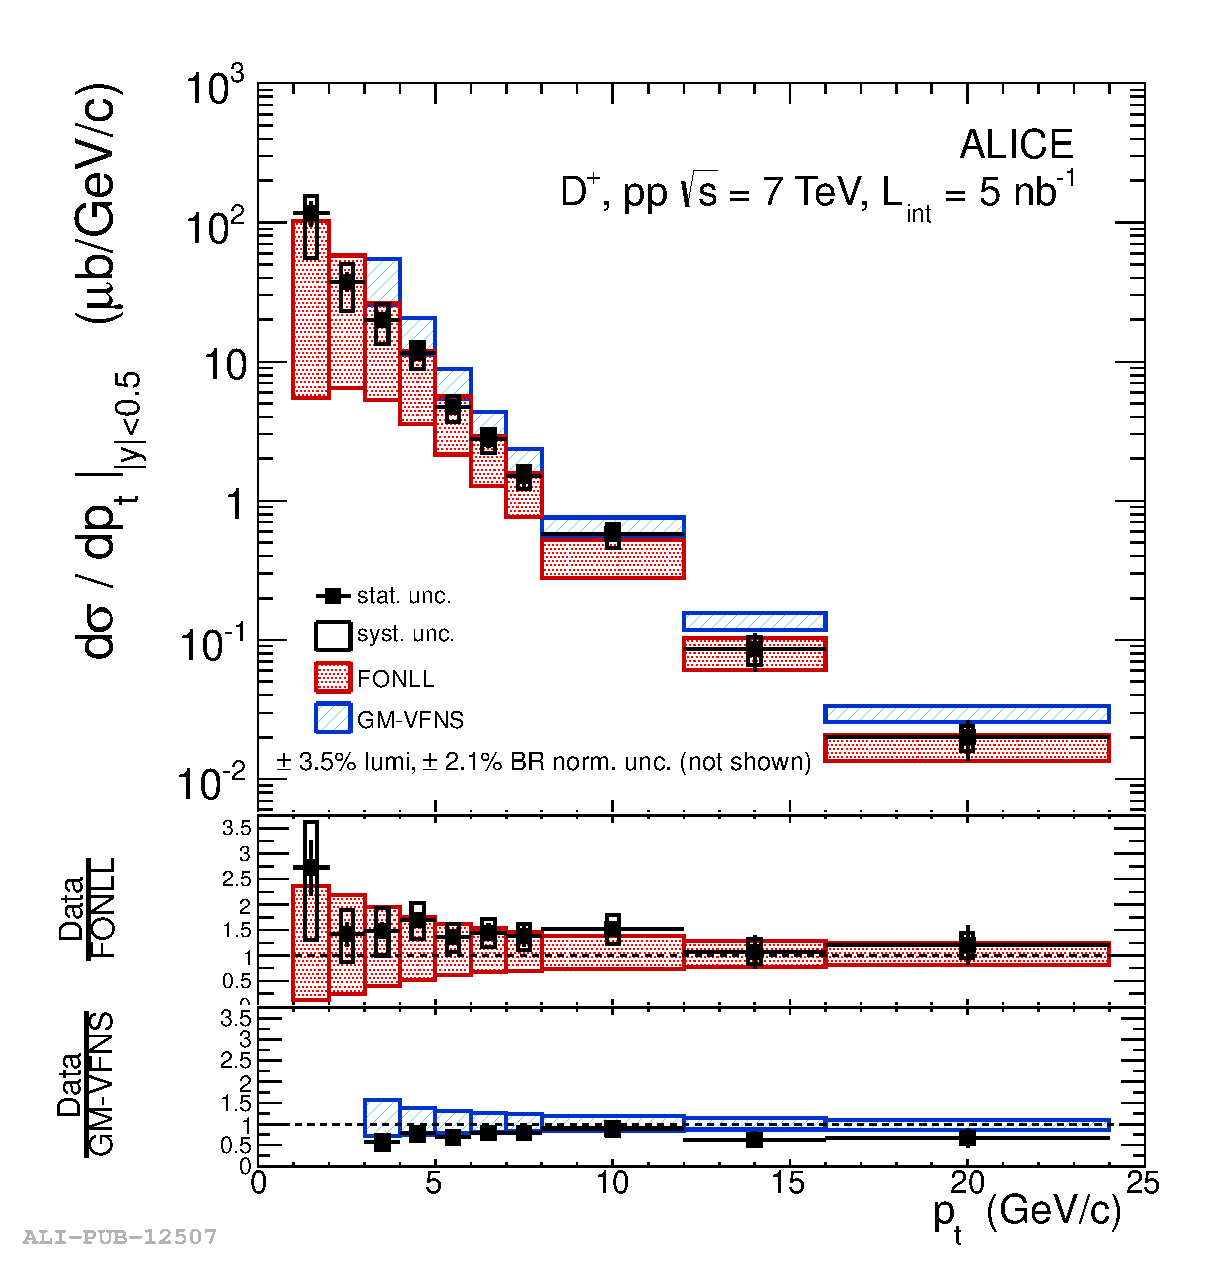
\includegraphics[scale=0.3]{2012-Jun-06-DplusCrossSection_pp7TeV.eps}}
\put(175,85){\includegraphics[scale=0.3]{jpsi_nonprompt_LHCb.png}}

\put(10,50){\captionsetup{labelformat=empty}
\begin{minipage}[t]{0.9\linewidth}
\begin{center}
Le sezioni d'urto per adroni contenenti $charm$ e $bottom$ misurate in collisioni pp sono in accordo con la predizione di FONLL \\$\Rightarrow$ nei metodi \textit{theory-driven} la sezione d'urto è calcolata utilizzando FONLL
\end{center}
\end{minipage}}

\end{picture} 
\end{frame}

\section{Metodo del fit del parametro di impatto}
\begin{frame}
\frametitle{}
\begin{picture}(320,250)

\put(15,180){
\begin{minipage}[t]{0.9\linewidth}
\begin{block}{}
\begin{center}
\fontsize{0.8cm}{1.cm}\selectfont{\textcolor{blue}{Metodo I \\ Fit del parametro di impatto}}
\end{center}
\end{block}
\end{minipage}}

\end{picture}
\end{frame}

\begin{frame}
\frametitle{Parametro di impatto}
\begin{picture}(320,250)

\put(10,105){\includegraphics[scale=0.21]{Prompt_sketch.png}}
\put(180,100){\includegraphics[scale=0.16]{FD_sketch.png}}

\put(-3,250){\captionsetup{labelformat=empty}
\begin{minipage}[t]{1.\linewidth}
\begin{block}{Parametro di impatto $d_0$}
Minima distanza tra il prolungamento della traccia del mesone $D^+$ ed il vertice primario
\end{block}
\end{minipage}}

\put(-15,105){\captionsetup{labelformat=empty}
\begin{minipage}[t]{0.43\linewidth}
\begin{center}
\textcolor{blue}{$D^+$ prompt}\\ il parametro di impatto è nullo\\ $\Rightarrow$ ci aspettiamo quindi una distribuzione gaussiana a causa \\della risoluzione del rivelatore
\end{center}
\end{minipage}}

\put(142,95){\captionsetup{labelformat=empty}
\begin{minipage}[t]{0.59\linewidth}
\begin{center}
\textcolor{blue}{$D^+$ feed-down}\\ il parametro di impatto non è nullo, ma dipende dalla lunghezza di decadimento del mesone $B$ e dall'angolo tra la direzione di volo dei mesoni $B$ e $D$
\end{center}
\end{minipage}}

\put(0,35){\captionsetup{labelformat=empty}
\begin{minipage}[t]{1\linewidth}
$\Rightarrow$ per separare i due contributi si può perciò eseguire un fit sulle distribuzioni del parametro di impatto, in intervalli di momento trasverso $p_{T}$
\end{minipage}}

\end{picture} 
\end{frame}

\subsection{Procedimento}
\begin{frame}
\frametitle{Fit delle distribuzioni del parametro di impatto - procedimento}
\begin{picture}(320,250)

\put(0,235){\captionsetup{labelformat=empty}
\begin{minipage}[t]{0.95\linewidth}
\begin{enumerate}
 \item \textcolor{blue}{Prefit}
 \begin{itemize}
  \item Prefit sulle distribuzioni MC delle $D^+$ prompt
  \item Prefit sulle distribuzioni MC delle $D^+$ feed-down
  \item Prefit sulle distribuzioni del fondo ottenuta dai dati nella regione di massa invariante a lato del picco (\textit{sidebands})
 \end{itemize}
 \vspace{0.1cm}
  Nella fase di prefit si ottengono tutti i parametri che vengono successivamente fissati nel fit finale
 \vspace{0.2cm}
 \item \textcolor{blue}{Fit unbinned dei dati}\\
 La funzione di fit finale è somma dei singoli contributi
\vspace{1.6cm}

dove
\begin{itemize}
\item Tutti i parametri sono fissati dai prefit a meno di $f_{prompt}$ e il parametro di risoluzione $\sigma_{prompt}$
\item Il parametro $N_{sgn}$ è fissato al valore estratto dai fit di massa invariante (\textit{raw yield})
\item Il fattore di normalizzazione $N$ è fissato al numero totale di entrate
\end{itemize}

\end{enumerate}
\end{minipage}}

 \put(15,130){\captionsetup{labelformat=empty}
\begin{minipage}[t]{0.9\linewidth}
 \begin{block}{}
 \setlength\abovedisplayskip{0pt}
\[ F(d_0) = N_{sgn}\bigg\{f_{prompt}F_{prompt}(d_0)+(1-f_{prompt})F_{feeddown}(d_0) \bigg\} + (N-N_{sgn}) F_{bkg}(d_0)\]   
\end{block}
\end{minipage}}

\end{picture} 
\end{frame}

\subsection{Prefit sulle distribuzioni MC}
\begin{frame}
\frametitle{Distribuzione del parametro di impatto dei mesoni $D^+$ prompt}
\begin{picture}(320,250)

\put(0,235){\captionsetup{labelformat=empty}
\begin{minipage}[t]{1.\linewidth}
$\Rightarrow$ ottenuta da un sample di eventi MC p-Pb su cui sono stati applicati gli stessi tagli per la qualità delle tracce, tagli topologici e PID usati nell'analisi dei dati
\end{minipage}}

\put(12,220){\captionsetup{labelformat=empty}
\begin{minipage}[t]{0.92\linewidth}
\begin{block}{}
\[F_{prompt}(d_0) = N_{prompt}\bigg\{\frac{f_{gauss}}{\sqrt{2\pi}\sigma_{prompt}}e^{-\frac{(d_0-\mu_{prompt})^2}{2\sigma_{prompt}^2}}+\frac{(1-f_{gauss})}{2\lambda_{prompt}}e^{-\frac{|d_0-\mu_{prompt}|}{\lambda_{prompt}}}\bigg\}\]
\end{block}
\end{minipage}}

\put(10,15){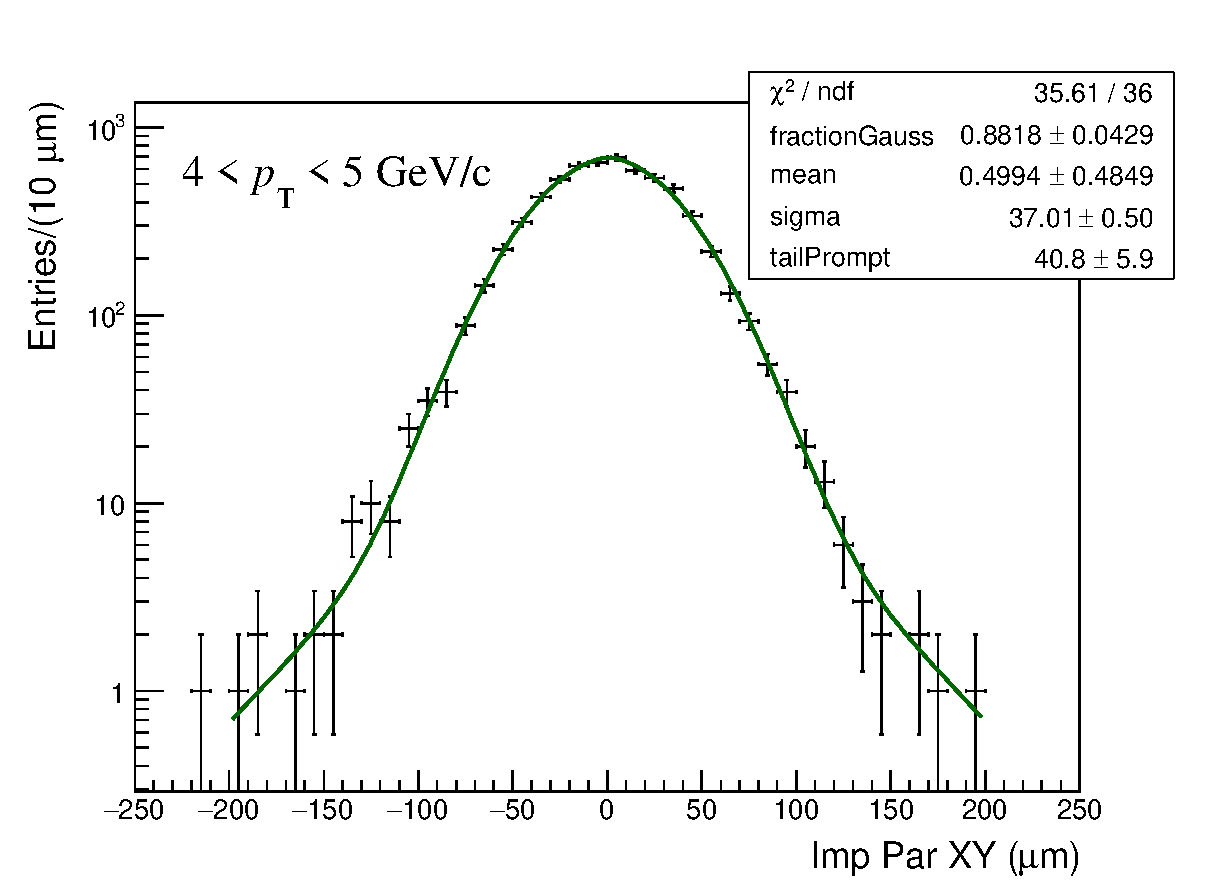
\includegraphics[scale=0.35]{ImpParPrompt_4-5.eps}}

\put(210,145){\captionsetup{labelformat=empty}
\begin{minipage}[t]{0.35\linewidth}
\begin{center}
Il fit alla distribuzione del parametro di impatto per le $D^+$ è stata eseguita con una funzione gaussiana con code esponenziali, per tener conto delle code non gaussiane\\\vspace{0.2cm}
$\Rightarrow$ siccome il parametro di impatto vero è nullo $\sigma_{prompt}$ ci fornisce una stima della risoluzione del rivelatore 
\end{center}
\end{minipage}}

\end{picture} 
\end{frame}

\begin{frame}
\frametitle{Distribuzione del parametro di impatto dei mesoni $D^+$ feed-down I}
\begin{picture}(320,250)

\put(0,235){\captionsetup{labelformat=empty}
\begin{minipage}[t]{1.\linewidth}
Due step per la parametrizzazione della distribuzione delle $D^+$ feed-down:
\begin{enumerate}
 \item fit della distribuzione del parametro di impatto \textit{vero} (non ricostruito) conosciuto dalla verità MC
 %\item convoluzione della funzione ottenuta dallo step precedente con $F_{prompt}(d_0)$
\end{enumerate}
\end{minipage}}

\put(10,15){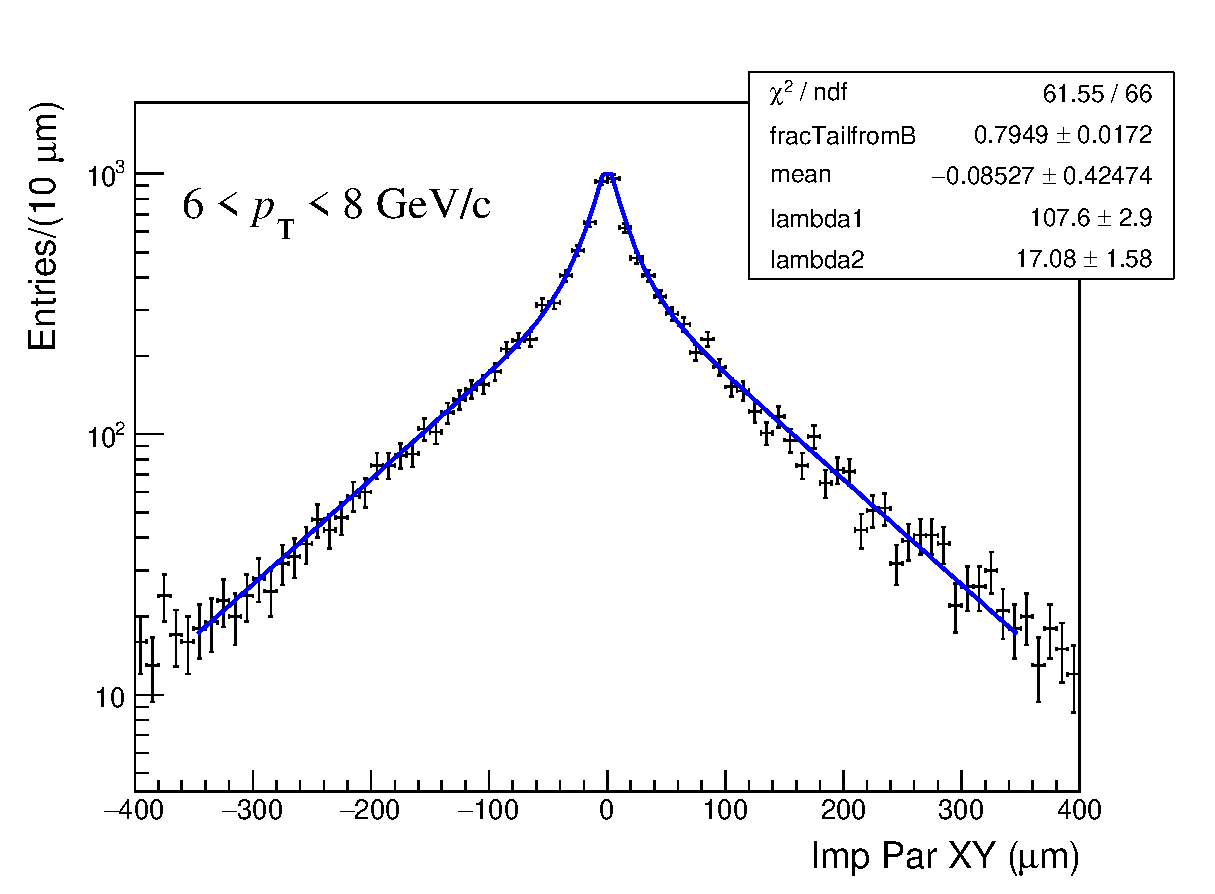
\includegraphics[scale=0.35]{ImpParTrueFD_6-8.eps}}

\put(15,210){\captionsetup{labelformat=empty}
\begin{minipage}[t]{0.9\linewidth}
 \begin{block}{}
\[F_{feeddown}^{true}(d_0) = N_{feeddown}\bigg\{\frac{f_{\lambda_1}}{2\lambda_1}e^{-\frac{|d_0-\mu_{feeddown}|}{\lambda_1}}+\frac{(1-f_{\lambda_1})}{2\lambda_2}e^{-\frac{|d_0-\mu_{feeddown}|}{\lambda_2}}\bigg\}\]
\end{block}
\end{minipage}}

\put(210,125){\captionsetup{labelformat=empty}
\begin{minipage}[t]{0.35\linewidth}
\begin{center}
Il parametro di impatto vero delle $D^+$ feed-down non è in generale nullo, per questo la loro distribuzione è stata fittata con una somma di due funzioni esponenziali, simmetrizzate rispetto al valor medio
\end{center}
\end{minipage}}

\end{picture} 
\end{frame}

\begin{frame}
\frametitle{Distribuzione del parametro di impatto dei mesoni $D^+$ feed-down II}
\begin{picture}(320,250)

\put(0,235){\captionsetup{labelformat=empty}
\begin{minipage}[t]{1.\linewidth}
Due step per la parametrizzazione della distribuzione delle $D^+$ feed-down:
\begin{enumerate}
\addtocounter{enumi}{1}
 %\item fit della distribuzione del parametro di impatto \textit{vero} (non ricostruito) conosciuto dalla verità MC
 \item convoluzione della funzione ottenuta dallo step precedente con $F_{prompt}(d_0)$
\end{enumerate}
\end{minipage}}

\put(10,15){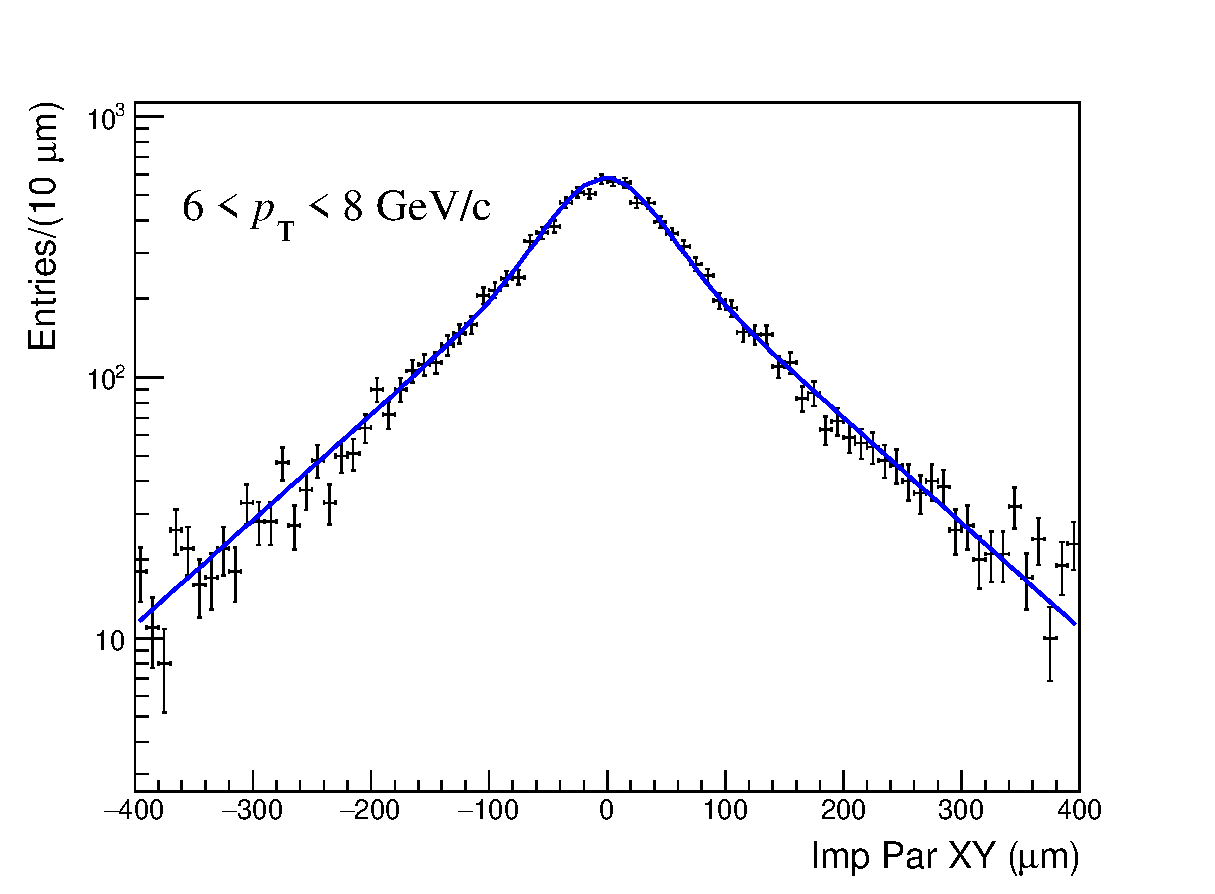
\includegraphics[scale=0.35]{ImpParRecoFD_6-8.eps}}

\put(40,210){\captionsetup{labelformat=empty}
\begin{minipage}[t]{0.75\linewidth}
 \begin{block}{}
\[F_{feeddown}^{reco}(d_0) = N_{feeddown} \int_{d_0^{min}}^{d_0^{max}} F_{feeddown}^{true}(d_0')F_{prompt}(d_0-d_0')dd_0'\]
\end{block}
\end{minipage}}

\put(210,125){\captionsetup{labelformat=empty}
\begin{minipage}[t]{0.35\linewidth}
\begin{center}
Per ottenere la parametrizzazione della distribuzione del parametro di impatto ricostruito si convolve la funzione $F^{true}_{feeddown}$ con $F_{prompt}$, che descrive l'allargamento a causa della risoluzione, fissando i parametri ottenuti nei fit precedenti
\end{center}
\end{minipage}}

\end{picture} 
\end{frame}

\subsection{Sidebands}

\begin{frame}
\frametitle{Distribuzione del parametro di impatto del fondo - \textit{Sidebands}}
\begin{picture}(320,250)

\put(10,120){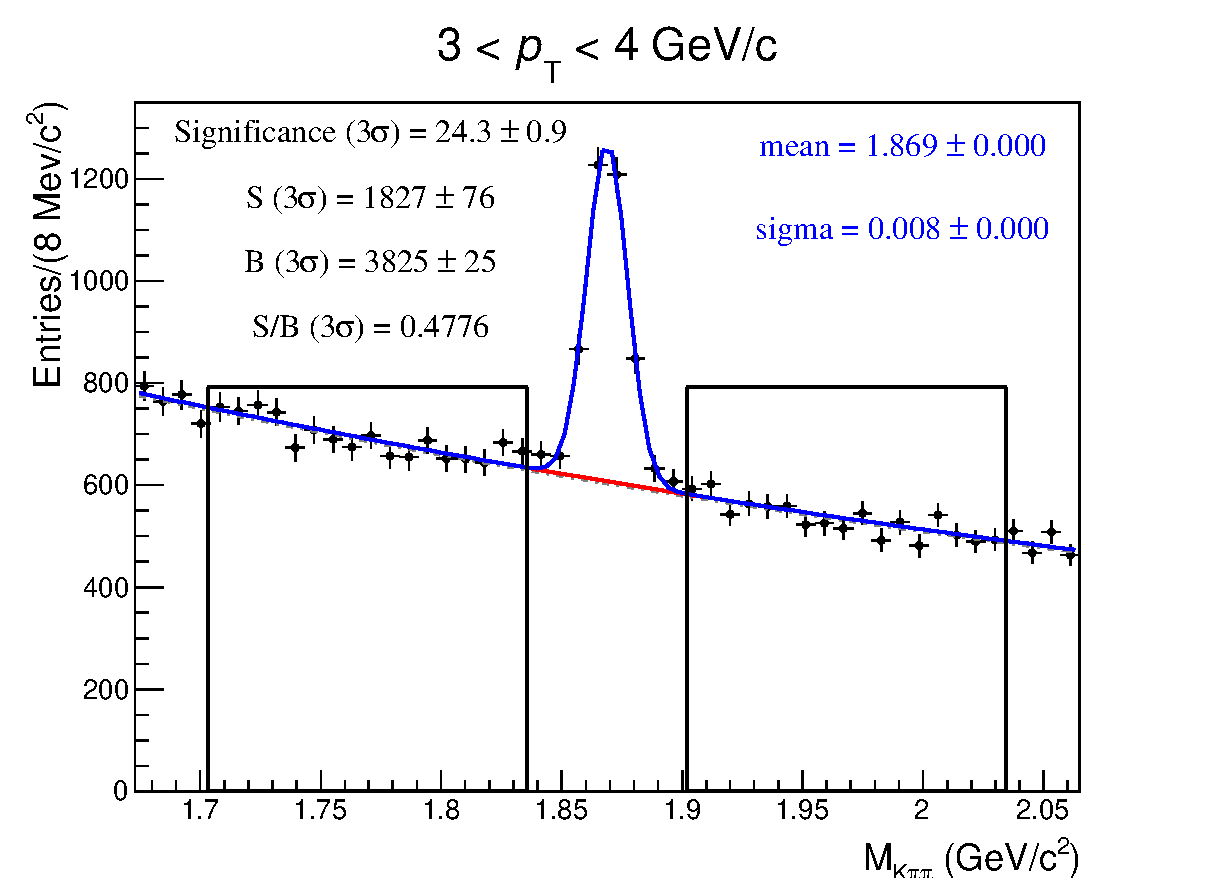
\includegraphics[scale=0.3]{Mass_3-4.eps}}
\put(180,15){\includegraphics[scale=0.3]{ImpParBkg_3-4_NoFit.eps}}

\put(150,130){
\begin{tikzpicture}[<-]
\draw[draw=black,solid,line width=0.2mm] (0, 0) -- + (-1.5, 0.78);
\end{tikzpicture}}

\put(81,80){
\begin{tikzpicture}[<-]
\draw[draw=black,solid,line width=0.2mm] (0, 0) -- + (-3.75, 2.34);
\end{tikzpicture}}

\put(180,230){\captionsetup{labelformat=empty}
\begin{minipage}[t]{0.45\linewidth}
\begin{center}
La distribuzione del parametro di impatto del fondo è ottenuta dai dati, considerando le regioni di massa invariante a lato del picco della $D^+$, in cui non è presente il segnale
\[|M-M_{PEAK}|> 4 \sigma\]
$\Rightarrow$ distribuzione delle \textit{sidebands}
\end{center}
\end{minipage}}

\put(20,80){\captionsetup{labelformat=empty}
\begin{minipage}[t]{0.4\linewidth}
\begin{center}
La distribuzione delle \textit{sidebands} fornisce una stima del fondo anche nella regione del picco di massa invariante
\end{center}
\end{minipage}}

\put(0,230){\captionsetup{labelformat=empty}
\begin{minipage}[t]{1.\linewidth}
\end{minipage}}

\end{picture} 
\end{frame}

\begin{frame}
\frametitle{Distribuzione del parametro di impatto del fondo - Fit}
\begin{picture}(320,250)

\put(5,240){\captionsetup{labelformat=empty}
\begin{minipage}[t]{0.95\linewidth}
 \begin{block}{}
 \setlength\abovedisplayskip{0pt}
\[F_{bkg}(d_0) = N_{bkg}\bigg\{F_{g+exp}(d_0;\text{ } f^{gauss}_{bkg},\mu_1^{bkg},\sigma_{bkg},\lambda_{bkg}) + F_{g+exp}(d_0;\text{ } f^{gauss}_{bkg},\mu_2^{bkg},\sigma_{bkg},\lambda_{bkg})\bigg\} \]
\end{block}
\end{minipage}}

\put(0,25){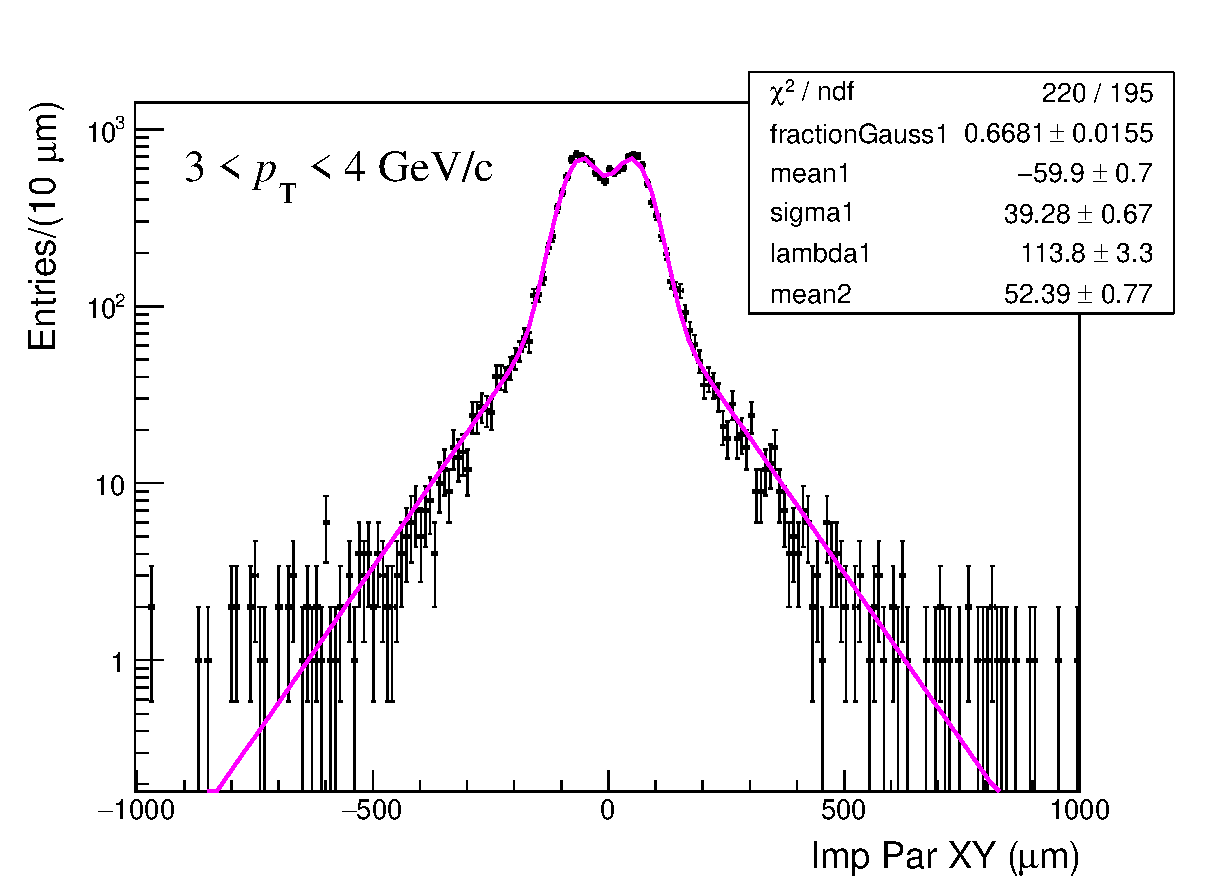
\includegraphics[scale=0.4]{ImpParBkg_3-4.eps}}

\put(230,145){\captionsetup{labelformat=empty}
\begin{minipage}[t]{0.3\linewidth}
\begin{center}
 La funzione utilizzata per il fit è la somma di due gaussiane con code esponenziali $F_{g+exp} (d_0)$, con tutti i parametri uguali a meno dei valori medi, per eliminare gli effetti di asimmetria dovuti a fluttuazioni statistiche
\end{center}
\end{minipage}}

\end{picture} 
\end{frame}

\subsection{Unbinned fit sui dati}
\begin{frame}
\frametitle{Unbinned fit sui dati I}
\begin{picture}(320,250)

\put(0,230){\captionsetup{labelformat=empty}
\begin{minipage}[t]{1.\linewidth}
La tecnica scelta per effettuare il fit sulla distribuzione del parametro di impatto dei dati è il \textit{\textcolor{blue} {fit unbinned}}
\end{minipage}}

\put(0,210){\captionsetup{labelformat=empty}
\begin{minipage}[t]{0.47\linewidth}
 \begin{block}{\centering Fit unbinned}
\setlength\abovedisplayskip{0pt}
 \[\ln{L(\theta_j)} = \sum_{i=1}^{n_{tot}} \ln{f(x_i,\theta_j)}\]
  \begin{center}
  $n_{tot} \rightarrow $ numero totale di misure\\
  $f(x_i,\theta_j)\rightarrow$  densità di probabilità di $x_i$ 
  \end{center}
\end{block}
\end{minipage}}

\put(177,210){\captionsetup{labelformat=empty}
\begin{minipage}[t]{0.47\linewidth}
 \begin{block}{\centering Fit binned}
\setlength\abovedisplayskip{0pt}
\[\ln{L(\theta_j)} = \sum_{i=1}^{N_{bins}} n_i\ln{\nu_i(\theta_j)}\]
\begin{center}
$N_{bins} \rightarrow$ numero di bin dell'istogramma 
$n_i \rightarrow$ numero di entrate nel bin  $i$-esimo\\
$\nu_i = n_{tot}\int_{x_i^{min}}^{x_i^{max}}f(x,\theta_{j})dx$\\
\end{center}
\end{block}
\end{minipage}}

\put(0,85){\captionsetup{labelformat=empty}
\begin{minipage}[t]{1.\linewidth}
\begin{center}
Il \textit{fit unbinned} permette di eliminare l'incertezza dovuta alla dimensione finita delle celle di un istogramma e di avere una migliore precisione nelle regioni in cui si hanno pochi conteggi
\end{center}
\end{minipage}}

\put(0,40){\captionsetup{labelformat=empty}
\begin{minipage}[t]{1.\linewidth}
\begin{center}
$\Rightarrow$ il fit non è perciò eseguito su un istogramma, ma su un \textit{\textcolor{blue}{tree}}, in cui i dati sono immagazzinati senza essere messi in bin, e che quindi permette di utilizzare il \textit{fit unbinned} 
\end{center}
\end{minipage}}

\end{picture} 
\end{frame}

\begin{frame}
\frametitle{Unbinned fit sui dati II}
\begin{picture}(320,250)

\put(0,140){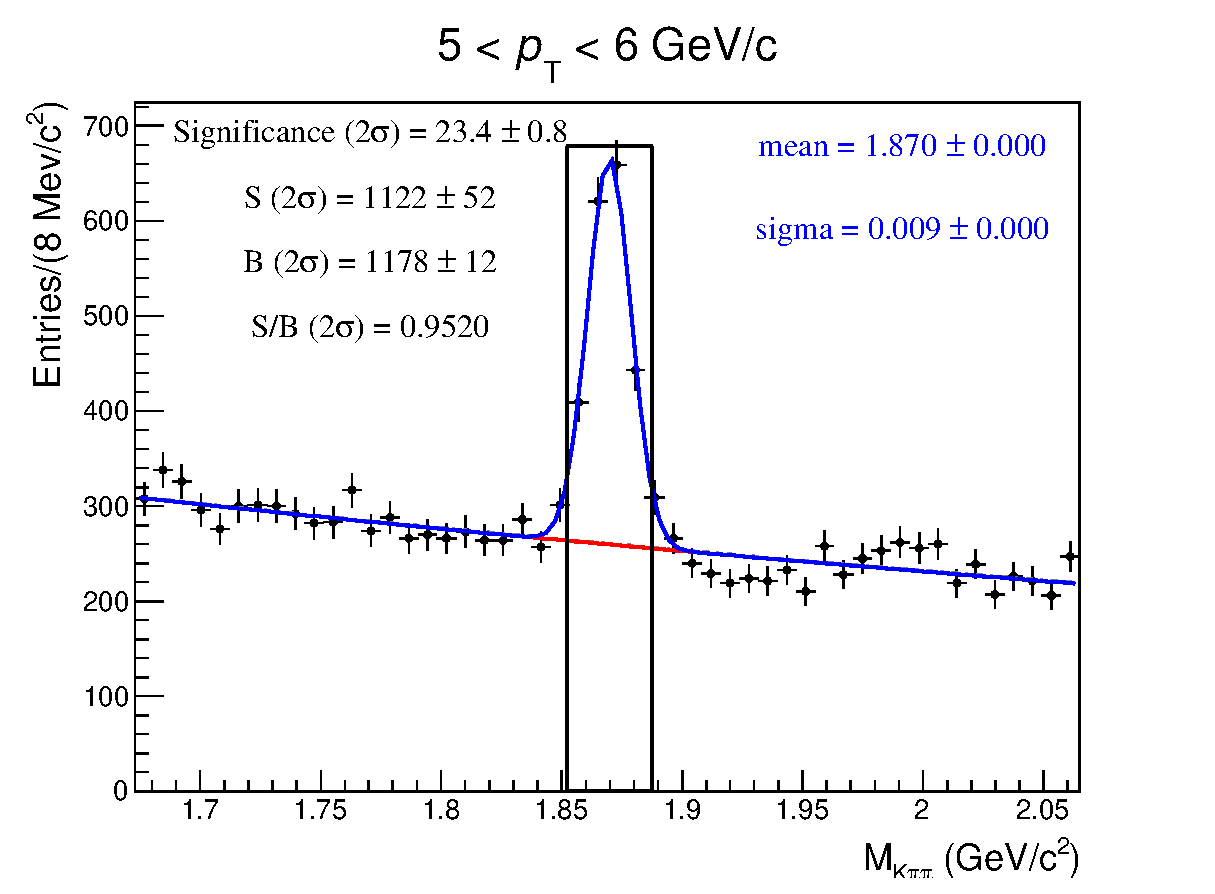
\includegraphics[scale=0.25]{Mass_5-6_fit.eps}}
\put(150,60){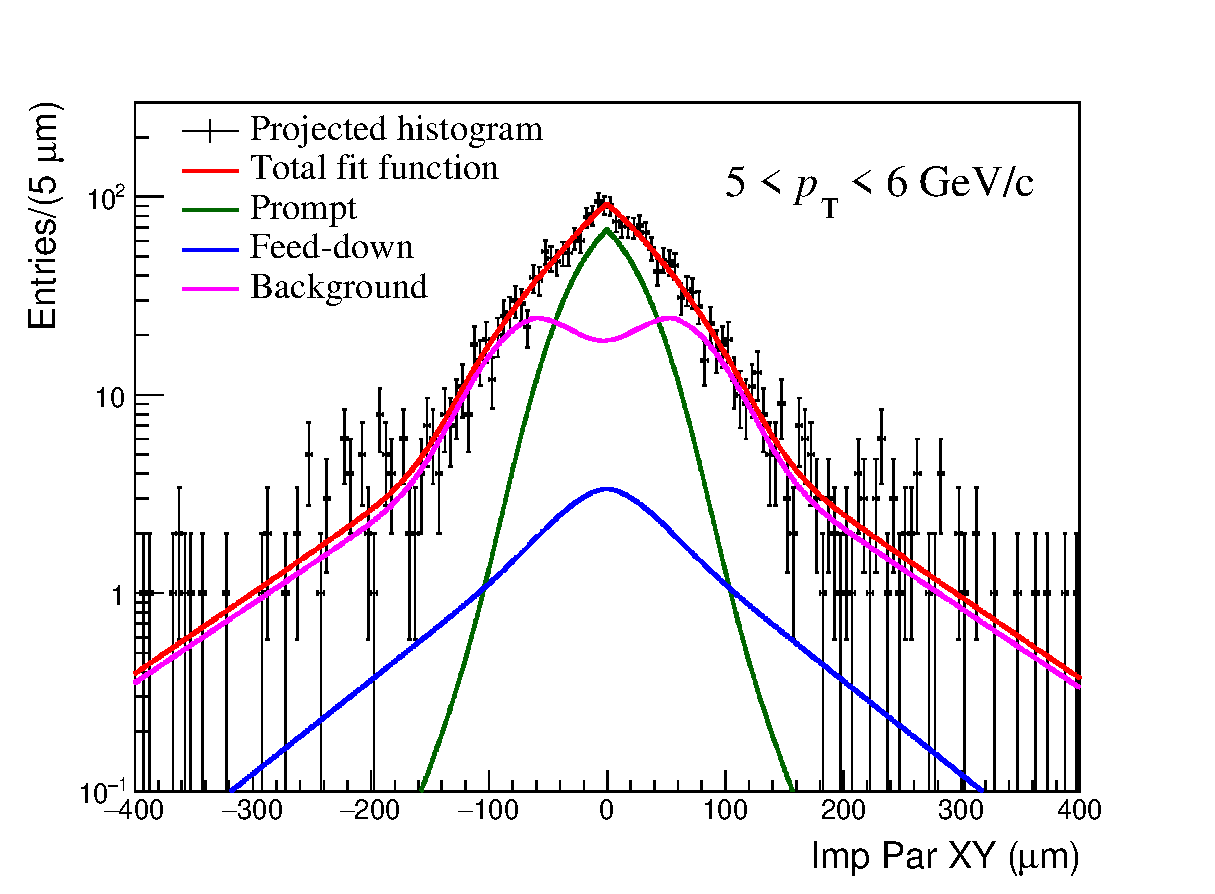
\includegraphics[scale=0.37]{FitUnbinned_5-6_bkg_plot.eps}}

\put(73.5,130){
\begin{tikzpicture}[<-]
\draw[draw=black,solid,line width=0.2mm] (0, 0) -- + (-2.95, 1.5);
\end{tikzpicture}}

\put(150,235){\captionsetup{labelformat=empty}
\begin{minipage}[t]{0.55\linewidth}
\begin{center}
La distribuzione del parametro di impatto dei dati è ottenuta considerando il range di massa invariante 
$|M-M_{PEAK}| < 2\sigma$
\end{center}
\end{minipage}}

\put(-10,130){\captionsetup{labelformat=empty}
\begin{minipage}[t]{0.45\linewidth}
\begin{itemize}
 \item Parametri liberi $\rightarrow f_{prompt}, \text{ } \sigma_{prompt}$
 \item $N_{sgn}$ è fissato al valore del segnale ottenuto dal fit della massa invariante (\textit{raw yield})
 \item $N$ è fissato al numero di entrate nel \textit{tree}
\end{itemize}
\end{minipage}}

\put(15,60){\captionsetup{labelformat=empty}
\begin{minipage}[t]{0.9\linewidth}
 \begin{block}{}
 \setlength\abovedisplayskip{0pt}
\[ F(d_0) = N_{sgn}\bigg\{f_{prompt}F_{prompt}(d_0)+(1-f_{prompt})F_{feeddown}^{reco}(d_0) \bigg\} + (N-N_{sgn}) F_{bkg}(d_0)\]   
\end{block}
\end{minipage}}

\end{picture} 
\end{frame}

\subsection{Errori sistematici}
\begin{frame}
\frametitle{Errori sistematici - $\sigma_{prompt}$ fissata}
\begin{picture}(320,250)

\put(30,225){\captionsetup{labelformat=empty}
\begin{minipage}[t]{0.45\linewidth}
\begin{center}
Sono stati rieseguiti i fit fissando il parametro $\sigma_{prompt}$ al valore ottenuto dal prefit sulla distribuzione MC delle $D^+$ prompt
\end{center}
\end{minipage}}

\put(-5,65){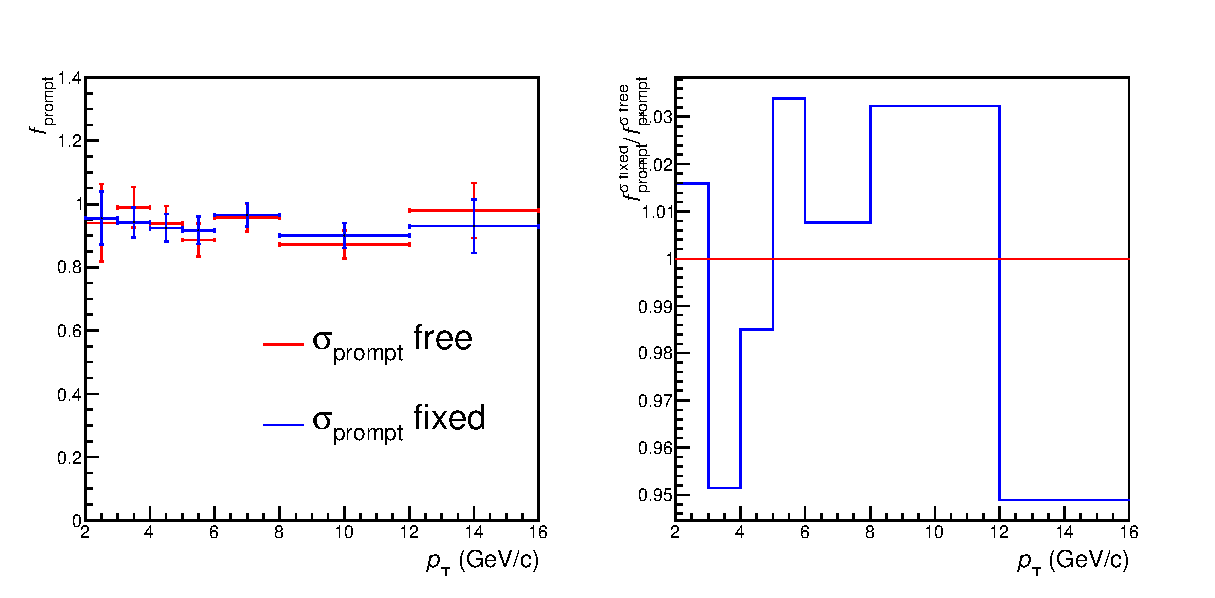
\includegraphics[scale=0.45]{promptfraction_syst_sigma.eps}}
\put(220,180){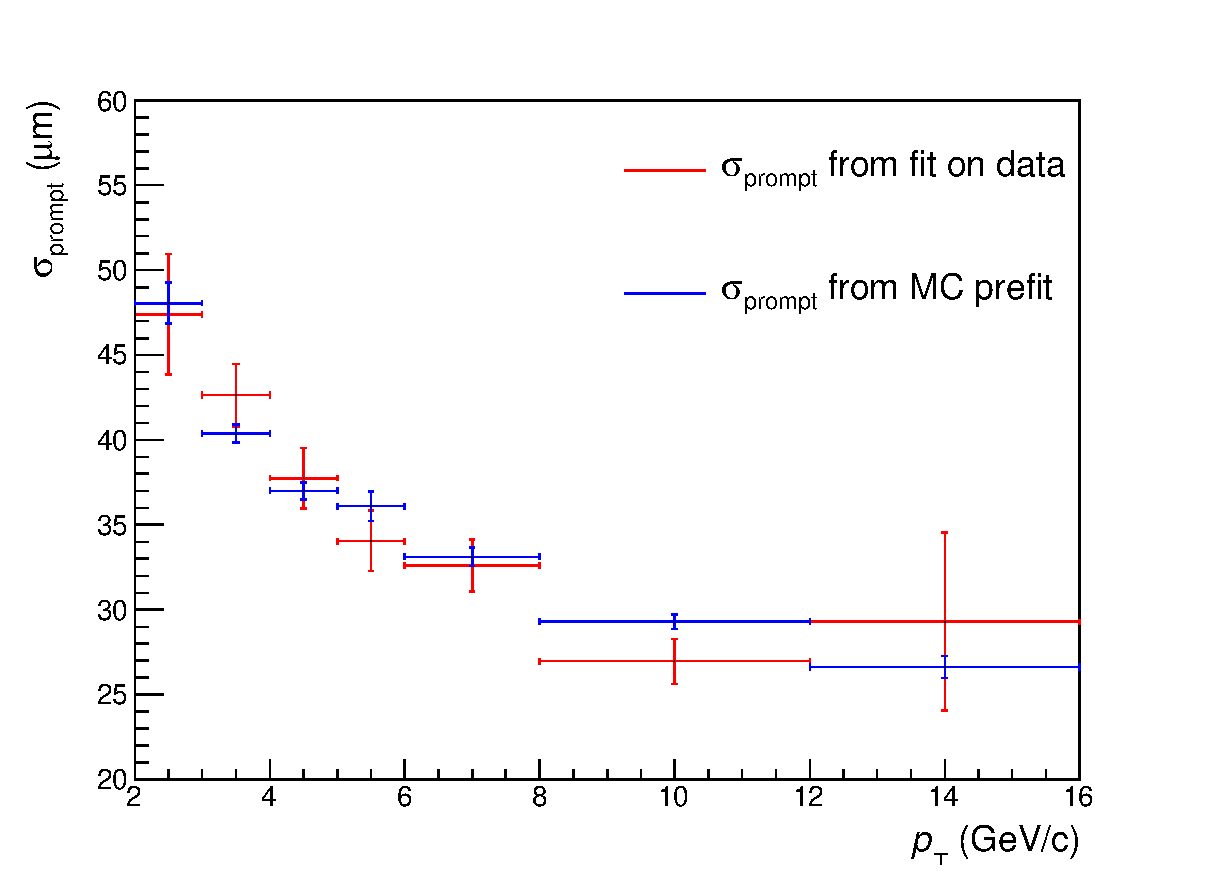
\includegraphics[scale=0.22]{sigmaprompt.eps}}

\put(250,160){\captionsetup{labelformat=empty}
\begin{minipage}[t]{0.25\linewidth}
\begin{center}
il valore ottenuto con $\sigma_{prompt}$ fissata oscilla intorno al risultato di riferimento\\
$\Rightarrow$ interpretato come fluttuazione statistica e perciò non considerato negli errori sistematici
\end{center}
\end{minipage}}

\put(20,35){\captionsetup{labelformat=empty}
\begin{minipage}[t]{0.36\linewidth}
\renewcommand\arraystretch{1.4} 
  \begin{tabular}{c|c|c|c|c|c|c|c}
    $p_T (GeV/c)$ & $2-3$ & $3-4$ & $4-5$ & $5-6$ & $6-8$ & $8-12$ & $12-16$ \\
    \hline
    $\sigma_{prompt}$ fissata & $0\%$ & $0\%$ & $0\%$ & $0\%$ & $0\%$ & $0\%$ & $0\%$ \\
  \end{tabular}
\end{minipage}}

\end{picture} 
\end{frame}

\begin{frame}
\frametitle{Errori sistematici - range del fit}
\begin{picture}(320,250)

\put(10,230){\captionsetup{labelformat=empty}
\begin{minipage}[t]{0.9\linewidth}
\begin{center}
Sono stati rieseguiti i fit e i prefit variando il range di parametro di impatto considerato, a partire da $[-200,200] \text{ } \mu m$ fino a $[-1000,1000] \text{ } \mu m$
\end{center}
\end{minipage}}

\put(-5,75){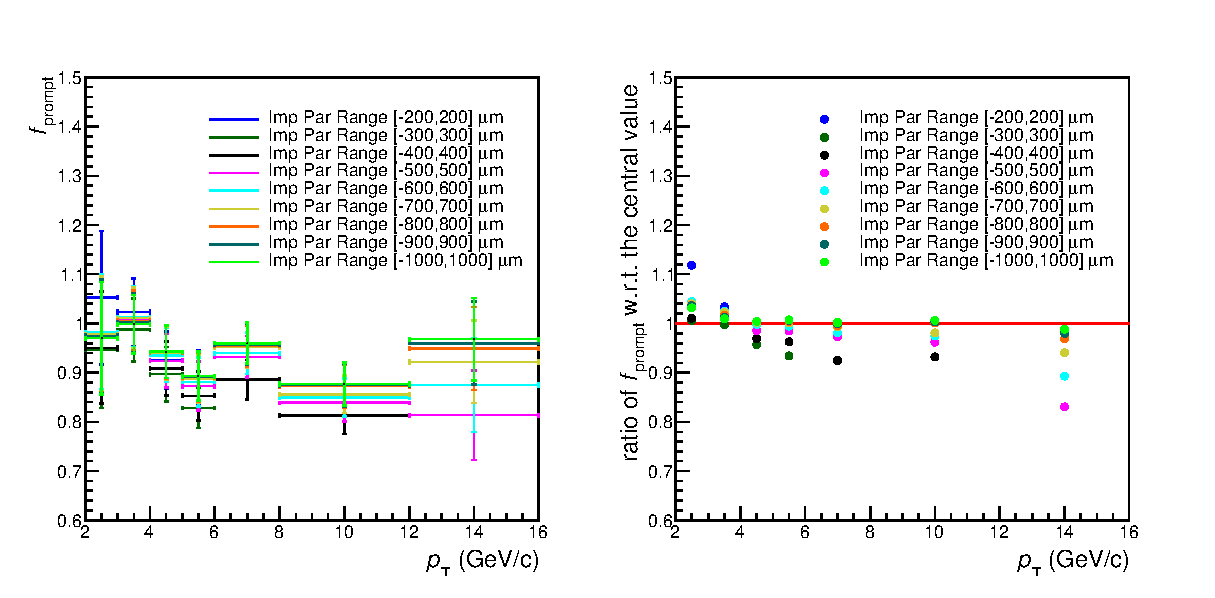
\includegraphics[scale=0.5]{promptfraction_syst_range.eps}}

\put(25,45){\captionsetup{labelformat=empty}
\begin{minipage}[t]{0.36\linewidth}
\renewcommand\arraystretch{1.4} 
  \begin{tabular}{c|c|c|c|c|c|c|c}
    $p_T (GeV/c)$ & $2-3$ & $3-4$ & $4-5$ & $5-6$ & $6-8$ & $8-12$ & $12-16$ \\
    \hline
    fit range & $2\%$ & $2\%$ & $2\%$ & $2\%$ & $2\%$ & $2\%$ & $2\%$ \\
  \end{tabular}
\end{minipage}}

\put(270,170){\captionsetup{labelformat=empty}
\begin{minipage}[t]{0.2\linewidth}
\begin{center}
In questo caso è stata valutata l'RMS della dispersione dei punti intorno al valore di riferimento 
\end{center}
\end{minipage}}

\end{picture} 
\end{frame}

\begin{frame}
\frametitle{Errori sistematici - regione di massa invariante}
\begin{picture}(320,250)

\put(10,230){\captionsetup{labelformat=empty}
\begin{minipage}[t]{0.9\linewidth}
\begin{center}
Sono stati rieseguiti i fit variando il range di massa invariante considerato da $|M-M_{PEAK}| < 1\sigma$ \hspace{0.05cm} a \hspace{0.05cm} $|M-M_{PEAK}| < 3\sigma$  
\end{center}
\end{minipage}}

\put(-5,75){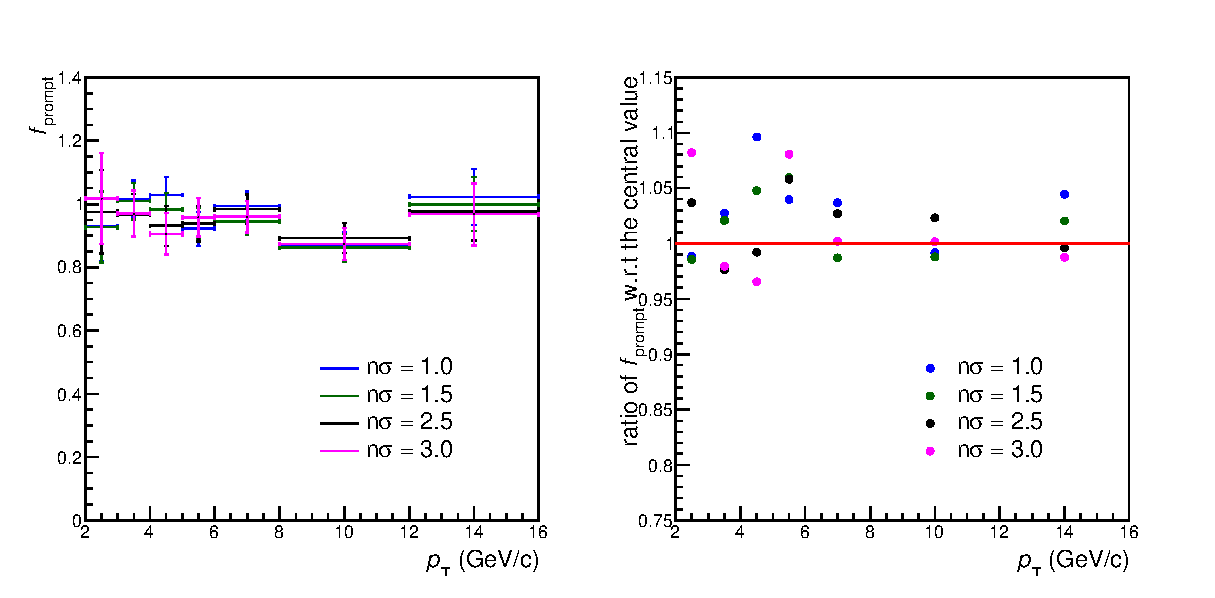
\includegraphics[scale=0.5]{promptfraction_syst_MassRange.eps}}

\put(15,45){\captionsetup{labelformat=empty}
\begin{minipage}[t]{0.36\linewidth}
\renewcommand\arraystretch{1.4} 
  \begin{tabular}{c|c|c|c|c|c|c|c}
    $p_T (GeV/c)$ & $2-3$ & $3-4$ & $4-5$ & $5-6$ & $6-8$ & $8-12$ & $12-16$ \\
    \hline
    range di massa& $0\%$ & $0\%$ & $0\%$ & $0\%$ & $0\%$ & $0\%$ & $0\%$ \\
  \end{tabular}
\end{minipage}}

\put(270,180){\captionsetup{labelformat=empty}
\begin{minipage}[t]{0.2\linewidth}
\begin{center}
Non c'è alcun trend osservato, nè un'evidente gerarchia tra i set di punti, perciò non è stato assegnato alcun errore sistematico 
\end{center}
\end{minipage}}

\end{picture} 
\end{frame}

\begin{frame}
\frametitle{Errori sistematici - regione di massa invariante delle \textit{sidebands}}
\begin{picture}(320,250)

\put(35,65){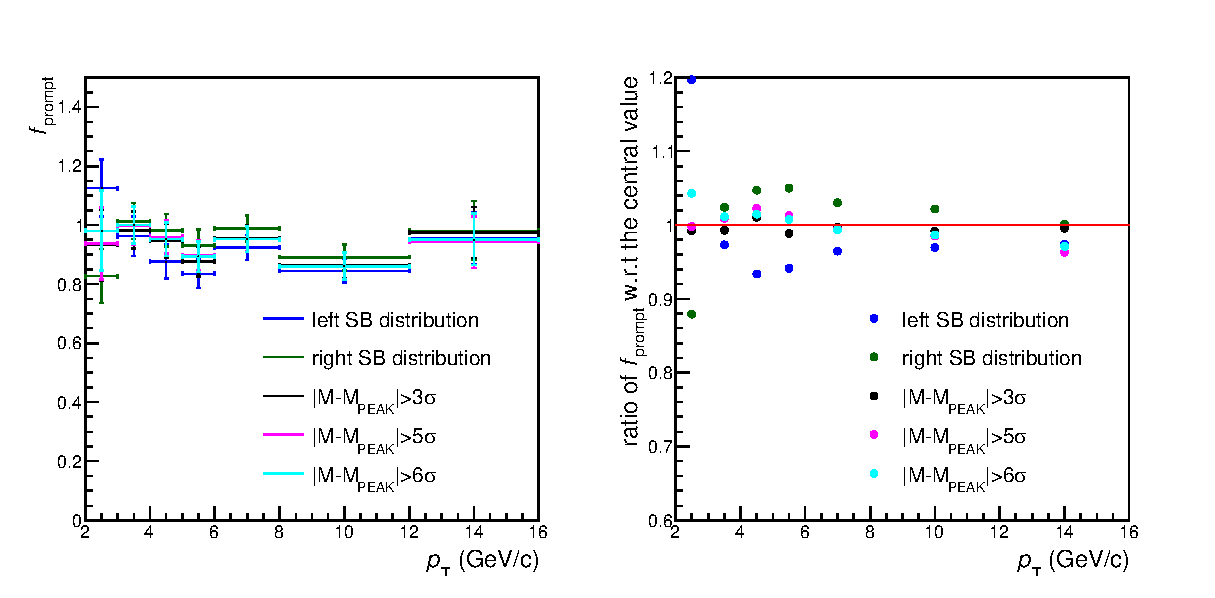
\includegraphics[scale=0.48]{promptfraction_syst_SBtot.eps}}

\put(10,235){\captionsetup{labelformat=empty}
\begin{minipage}[t]{0.9\linewidth}
Sono stati rieseguiti i fit variando il range di massa invariante considerato per la parametrizzazione delle \textit{sidebands}
\begin{itemize}
 \item intervalli simmetrici rispetto al picco $|M-M_{PEAK}|>n\sigma$
 \item regioni soltanto a destra e a sinistra del picco 
\end{itemize}
\end{minipage}}

\put(15,35){\captionsetup{labelformat=empty}
\begin{minipage}[t]{0.36\linewidth}
\renewcommand\arraystretch{1.4} 
  \begin{tabular}{c|c|c|c|c|c|c|c}
    $p_T (GeV/c)$ & $2-3$ & $3-4$ & $4-5$ & $5-6$ & $6-8$ & $8-12$ & $12-16$ \\
    \hline
    range delle SB & $6\%$ & $3\%$ & $3\%$ & $3\%$ & $3\%$ & $3\%$ & $3\%$ \\
  \end{tabular}
\end{minipage}}

\end{picture} 
\end{frame}

\begin{frame}
\frametitle{Errori sistematici - prefit alla distribuzione delle \textit{sidebands}}
\begin{picture}(320,250)

\put(35,65){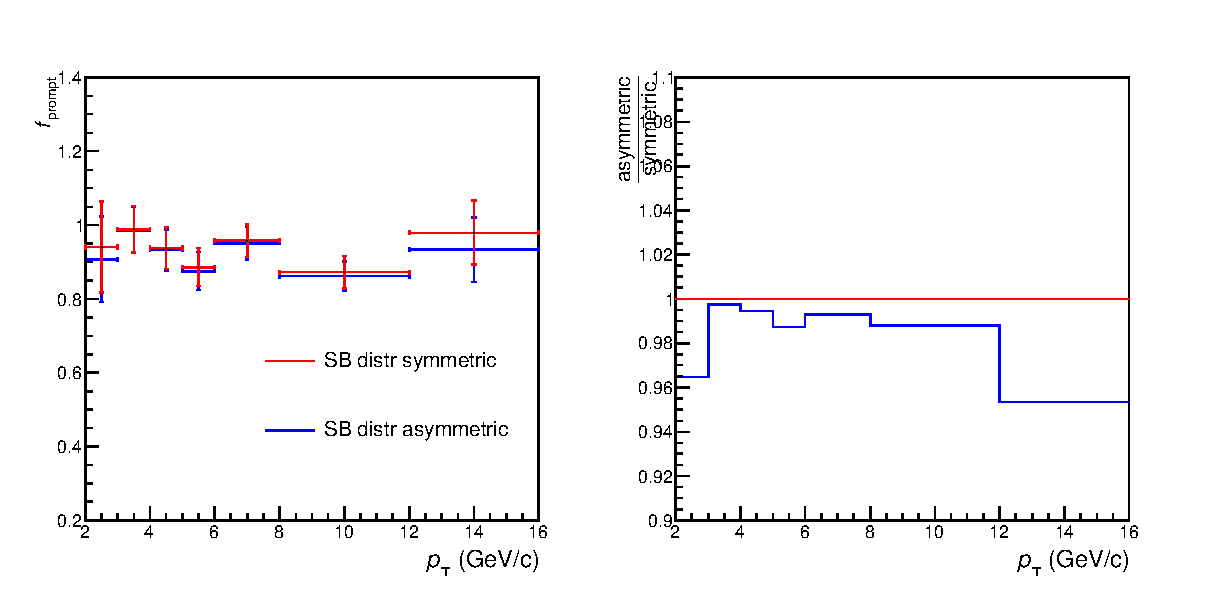
\includegraphics[scale=0.48]{promptfraction_syst_prefit.eps}}

\put(10,230){\captionsetup{labelformat=empty}
\begin{minipage}[t]{0.9\linewidth}
\begin{center}
Sono stati rieseguiti i fit utilizzando una funzione di fit asimmetrica per la distribuzione delle \textit{sidebands} (stessa funzione con i parametri delle due $F_{prompt}(d_0)$ indipendenti), per tener conto del fatto che l'asimetria rispetto a $d_0 = 0$ potrebbe non essere dovuta soltanto a fluttuazioni statistiche 
\end{center}
\end{minipage}}

\put(15,35){\captionsetup{labelformat=empty}
\begin{minipage}[t]{0.36\linewidth}
\renewcommand\arraystretch{1.4} 
  \begin{tabular}{c|c|c|c|c|c|c|c}
    $p_T (GeV/c)$ & $2-3$ & $3-4$ & $4-5$ & $5-6$ & $6-8$ & $8-12$ & $12-16$ \\
    \hline
    prefit delle SB & $4\%$ & $1\%$ & $1\%$ & $1\%$ & $1\%$ & $1\%$ & $1\%$ \\
  \end{tabular}
\end{minipage}}

\end{picture} 
\end{frame}

\begin{frame}
\frametitle{Errori sistematici - segnale I}
\begin{picture}(320,250)

\put(5,15){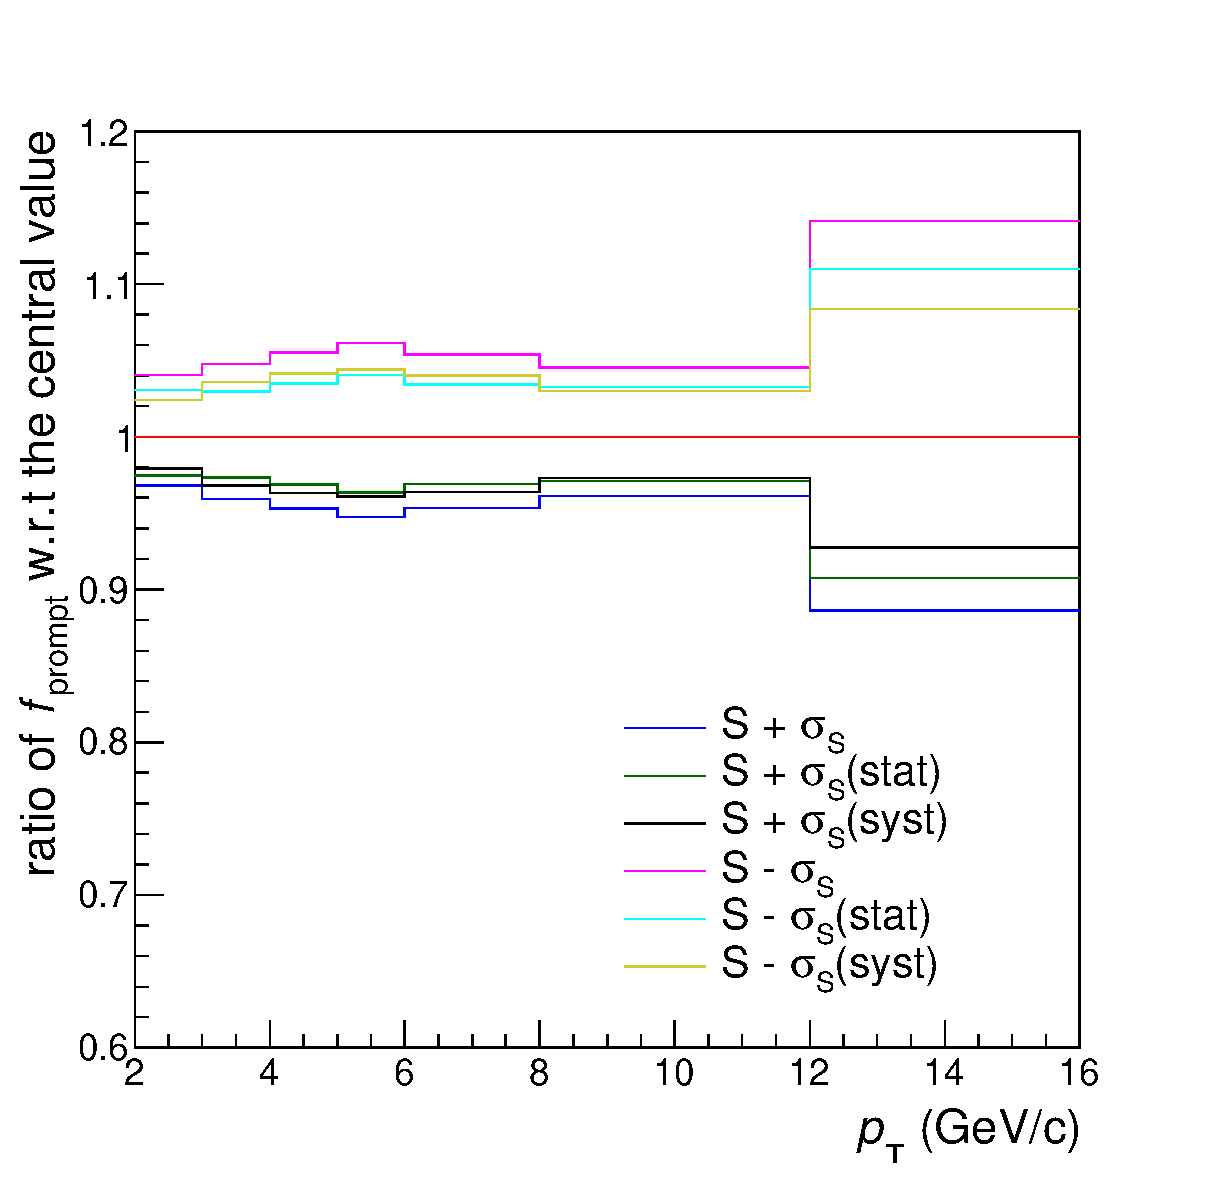
\includegraphics[scale=0.28]{fprompt_syst_SoverT_onlyratio.eps}}
\put(180,100){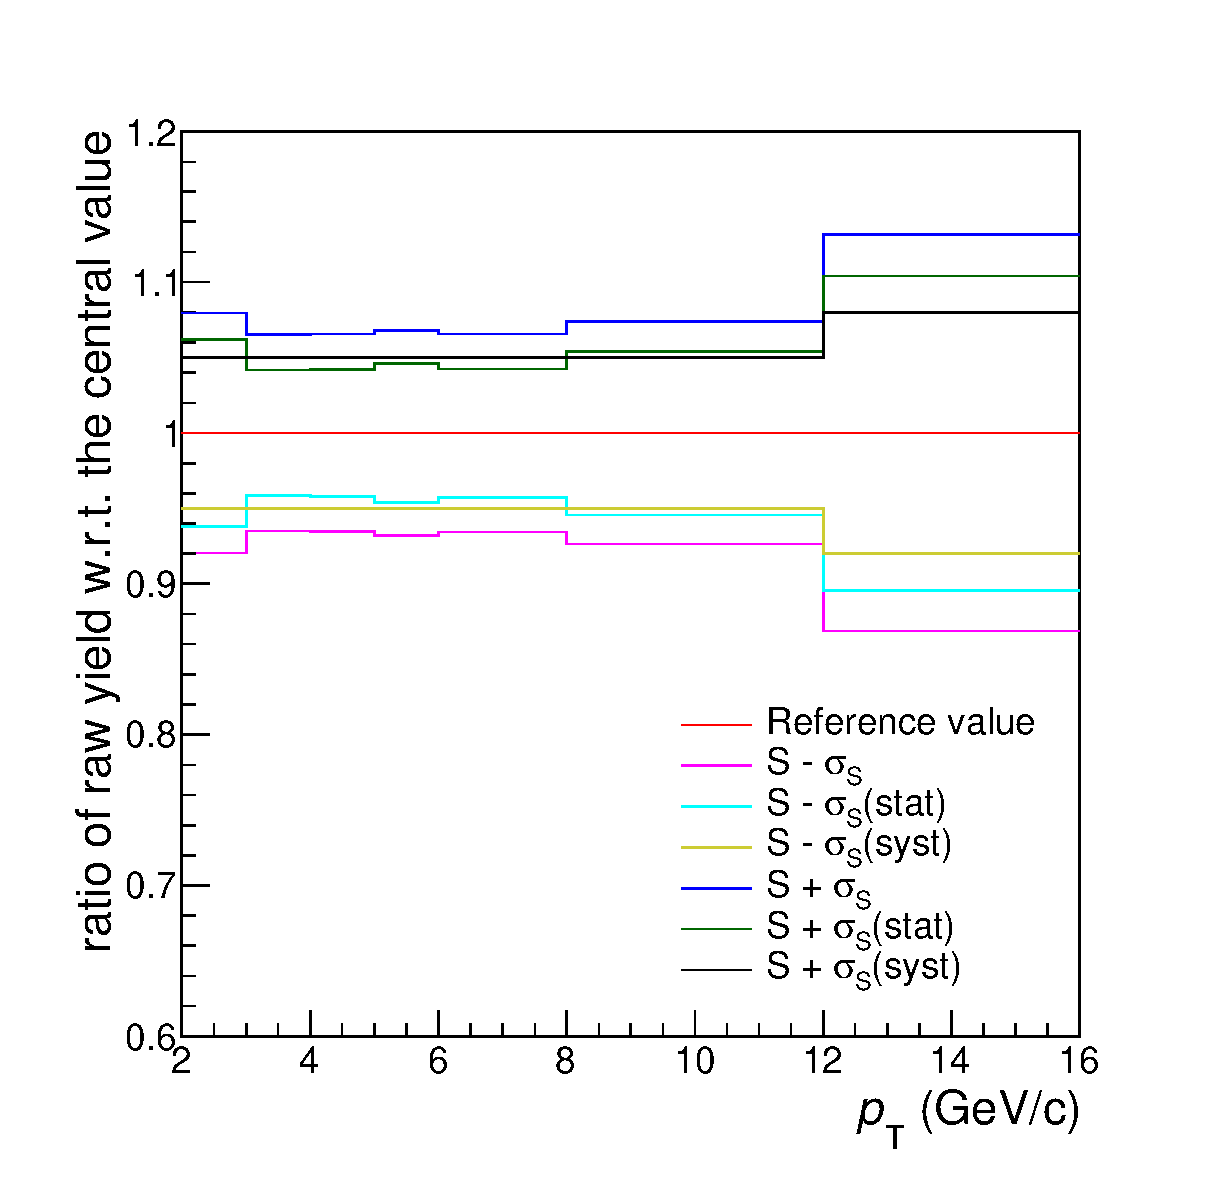
\includegraphics[scale=0.28]{rawyields_ratio.eps}}

\put(0,230){\captionsetup{labelformat=empty}
\begin{minipage}[t]{0.5\linewidth}
\begin{center}
Parametro $N_{sgn}$ fissato al valore di segnale $S$ estratto dai fit di massa invariante \\\vspace{0.2cm}
$\Rightarrow$ sono stati rieseguiti i fit fissando il parametro $N_{sgn}$ a $S\pm\sigma_{S}$, dove\\ 
$\sigma_S = \sqrt{\sigma_{S}^2(stat)+\sigma_{S}^2(syst)}$
\end{center}
\end{minipage}}

\put(165,80){\captionsetup{labelformat=empty}
\begin{minipage}[t]{0.5\linewidth}
\begin{center}
Aumento del segnale $\Rightarrow$ diminuzione della frazione di $D^{+}$ prompt\\\vspace{0.2cm}
Ci aspettiamo dunque un (parziale) cancellamento di questo errore nel calcolo della sezione d'urto
\end{center}
\end{minipage}}

\end{picture} 
\end{frame}

\begin{frame}
\frametitle{Errori sistematici - segnale II}
\begin{picture}(320,250)

\put(15,60){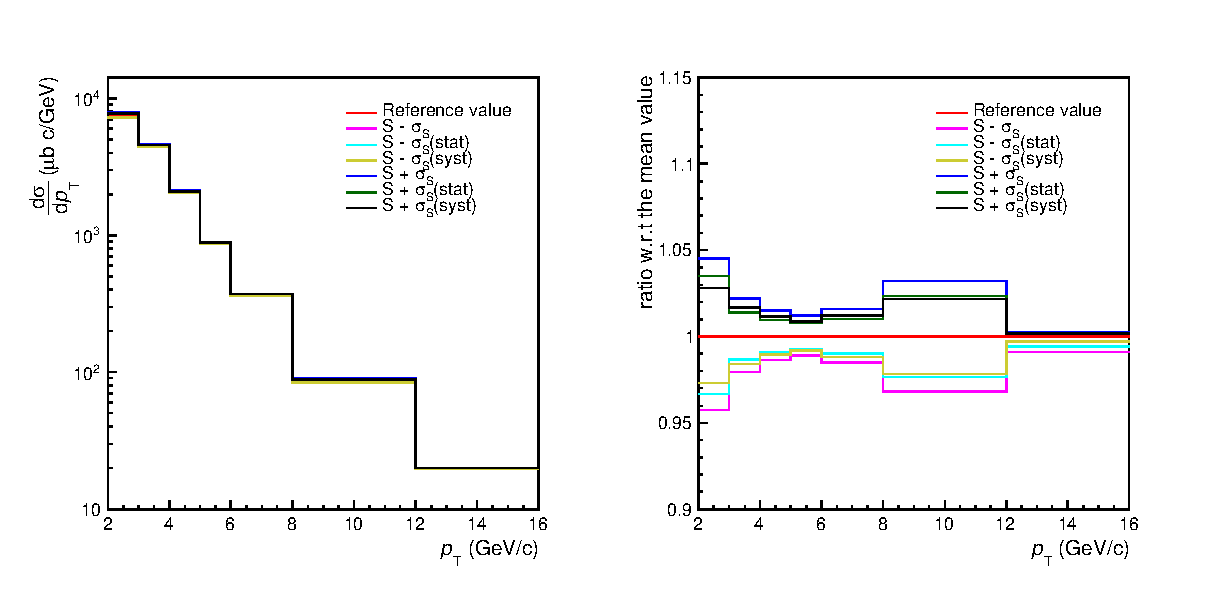
\includegraphics[scale=0.55]{promptcrosssection_syst_SoverT.eps}}

\put(10,250){\captionsetup{labelformat=empty}
\begin{minipage}[t]{0.55\linewidth}
\begin{block}{}
\setlength\abovedisplayskip{0pt}
 \[\frac{d\sigma_{prompt}^{D^+}}{dp_T} = \frac{\textcolor{blue}{f_{prompt}N^{D^+}_{raw}}}{2\Delta p_T \Delta y (\epsilon\times Acc)_{prompt}\cdot L_{int}\cdot BR}\]
\end{block}
\end{minipage}}
\put(200,225){\captionsetup{labelformat=empty}
\begin{minipage}[t]{0.4\linewidth}
\begin{center}
$\Rightarrow$ \hspace{0.1cm} parziale cancellazione\\ dell'errore 
\end{center}
\end{minipage}}

\put(25,40){\captionsetup{labelformat=empty}
\begin{minipage}[t]{0.36\linewidth}
\renewcommand\arraystretch{1.4} 
  \begin{tabular}{c|c|c|c|c|c|c|c}
    $p_T (GeV/c)$ & $2-3$ & $3-4$ & $4-5$ & $5-6$ & $6-8$ & $8-12$ & $12-16$ \\
    \hline
    segnale & $4\%$ & $2\%$ & $2\%$ & $2\%$ & $2\%$ & $2\%$ & $2\%$ \\
  \end{tabular}
\end{minipage}}

\end{picture} 
\end{frame}

\begin{frame}
\frametitle{Errori sistematici - forma della distribuzione in $p_T$ dei mesoni D e B}
\begin{picture}(320,250)

\put(5,235){\captionsetup{labelformat=empty}
\begin{minipage}[t]{0.65\linewidth}
\begin{center}
Lo spettro in $p_T$ dei mesoni D e B nel MC è leggermente diverso dallo spettro predetto da $FONLL$ \\
$\Rightarrow$ questo può introdurre un errore sistematico nei prefit dal momento che la risoluzione del parametro di impatto (e della lunghezza di decadimento per i mesoni $B$) dipende dal momento trasverso
\end{center}
\end{minipage}}

\put(-5,55){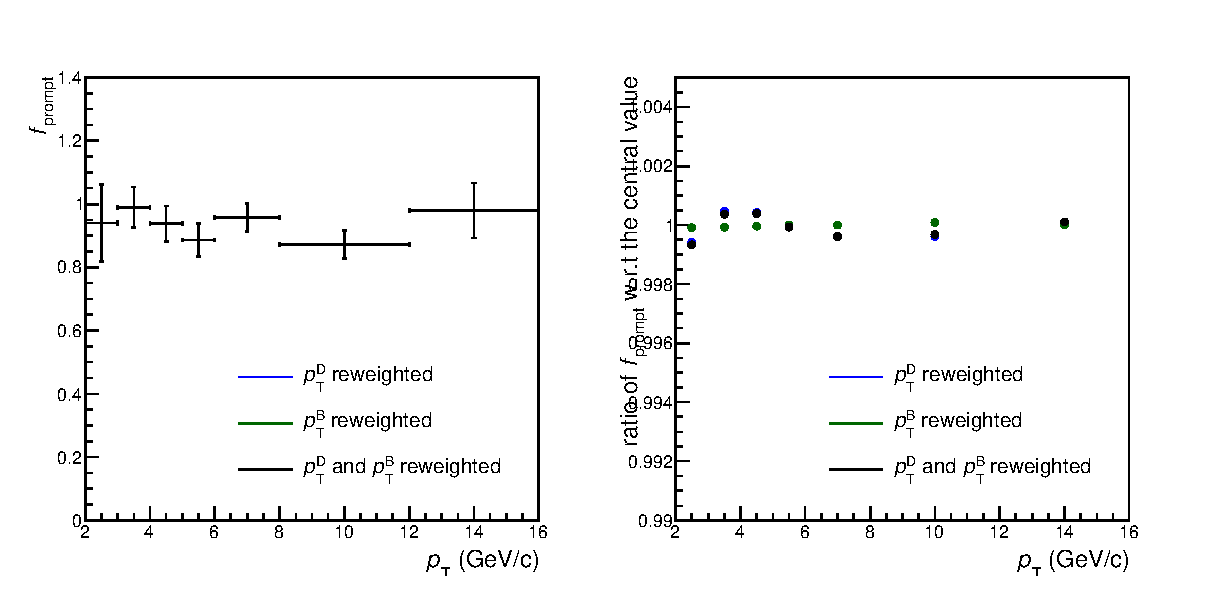
\includegraphics[scale=0.45]{promptfraction_syst_pTreweight.eps}}
\put(238,158){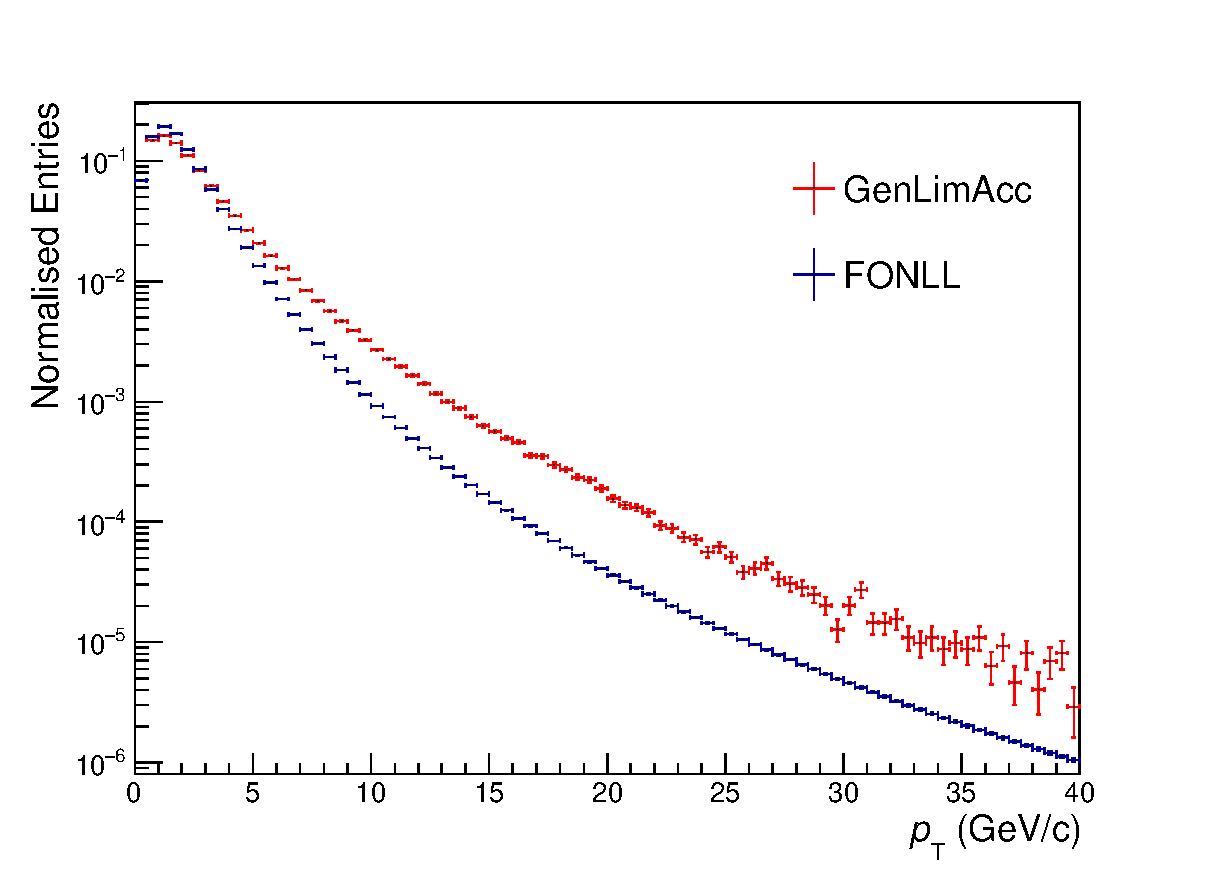
\includegraphics[scale=0.22]{DplusPrompt_PtSpectrum.eps}}

\put(250,140){\captionsetup{labelformat=empty}
\begin{minipage}[t]{0.25\linewidth}
\begin{center}
Le distribuzioni MC di $D^+$ prompt e feed-down sono state ripesate utilizzando gli spettri corretti dei mesoni D e B, e sono stati rieseguiti i fit
\end{center}
\end{minipage}}

\put(20,30){\captionsetup{labelformat=empty}
\begin{minipage}[t]{0.36\linewidth}
\renewcommand\arraystretch{1.4} 
  \begin{tabular}{c|c|c|c|c|c|c|c}
    $p_T (GeV/c)$ & $2-3$ & $3-4$ & $4-5$ & $5-6$ & $6-8$ & $8-12$ & $12-16$ \\
    \hline
    spettro in $p_T$& $0\%$ & $0\%$ & $0\%$ & $0\%$ & $0\%$ & $0\%$ & $0\%$ \\
  \end{tabular}
\end{minipage}}

\end{picture} 
\end{frame}

\subsection{MC closure test}
\begin{frame}
\frametitle{MC closure test}
\begin{picture}(320,250)

\put(0,65){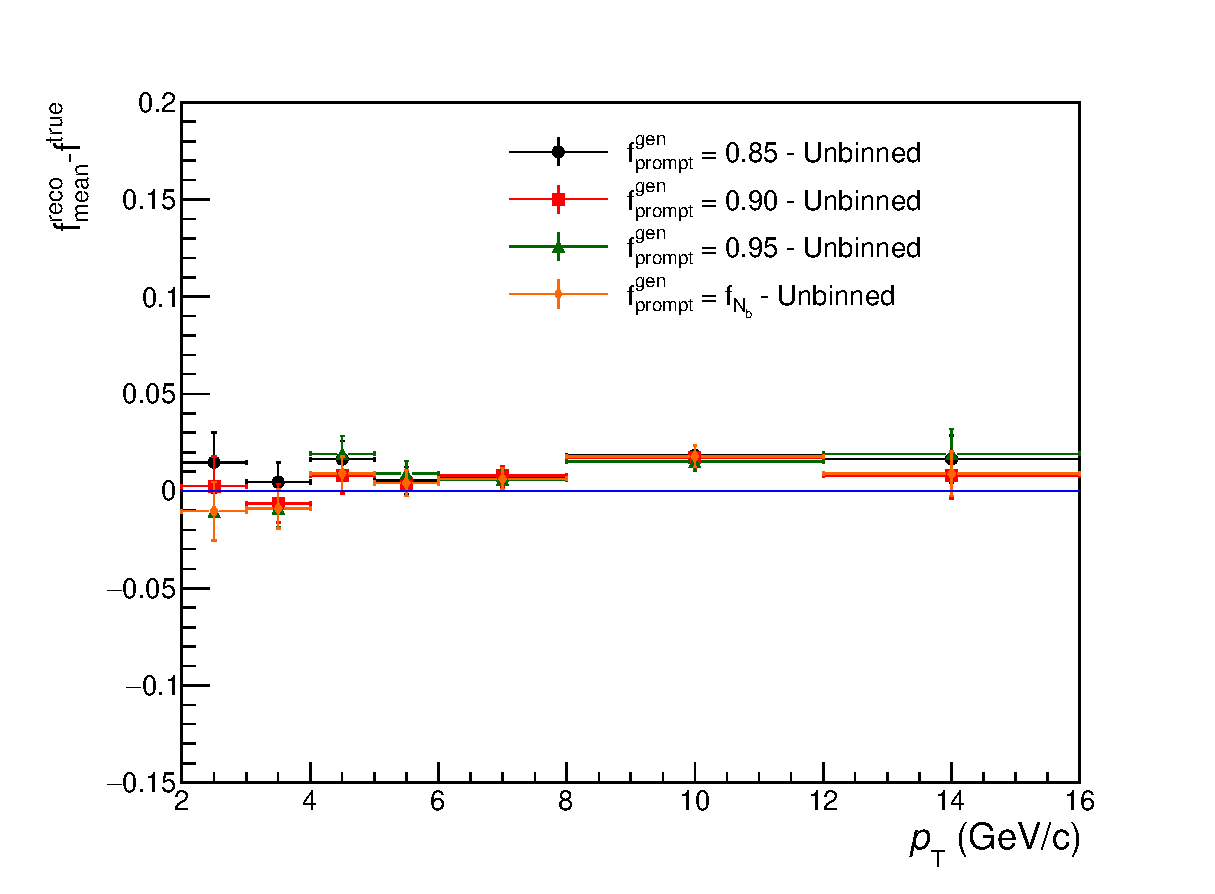
\includegraphics[scale=0.4]{Bias_bkg_freesigma.eps}}

\put(0,230){\captionsetup{labelformat=empty}
\begin{minipage}[t]{1.\linewidth}
\begin{center}
Per verificare la consistenza del metodo utilizzato è stato eseguito un \textcolor{blue}{test MC}
\end{center}
\end{minipage}}

\put(210,200){\captionsetup{labelformat=empty}
\begin{minipage}[t]{0.38\linewidth}
\begin{center}
I fit sono stati ripetuti 50 volte in ogni bin di momento trasverso, generando random le entrate dei tree a partire dalle distribuzioni MC per $D^+$ prompt e feed-down e dalle sidebands per il fondo \\\vspace{0.2cm}
\begin{itemize}
 \item numero di entrate per il segnale e il fondo fissate ai valori dei dati
 \item $f_{prompt}$ fissata arbitrariamente
\end{itemize}
\end{center}
\end{minipage}}

\put(0,50){\captionsetup{labelformat=empty}
\begin{minipage}[t]{1.\linewidth}
\begin{center}
I valori medi delle distribuzioni dei residui per $f_{prompt}$ tendono ad essere superiori a zero \\
$\Rightarrow$ si è assegnato un ulteriore $1\%$ all'errore sistematico, in ogni bin di $p_T$
\end{center}
\end{minipage}}

\end{picture} 
\end{frame}

\subsection{Risultato}
\begin{frame}
\frametitle{Frazione di $D^+$ prompt}
\begin{picture}(320,250)

\put(50,50){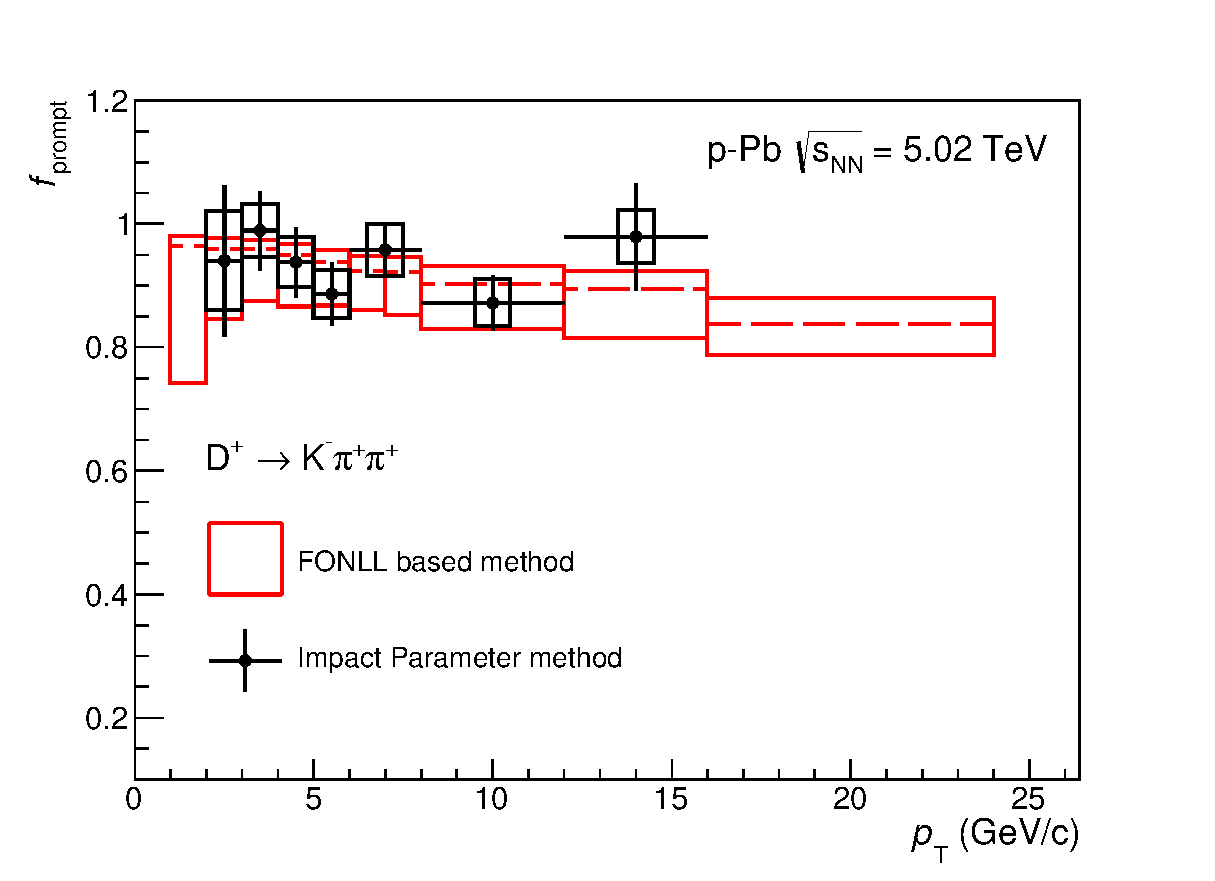
\includegraphics[scale=0.44]{prompt_fraction.eps}}

\put(10,235){\captionsetup{labelformat=empty}
\begin{minipage}[t]{0.9\linewidth}
\begin{center}
Il risultato ottenuto è in accordo con i metodi \textit{FONLL-based}, anche se con un'incertezza maggiore \\
\end{center}
\end{minipage}}

\put(10,35){\captionsetup{labelformat=empty}
\begin{minipage}[t]{0.9\linewidth}
\begin{center}
$\Rightarrow$ risultato inserito nell'articolo della produzione di mesoni D in collisioni pp e p-Pb come \textit{cross-check} dei metodi \textit{theory-driven}
\end{center}
\end{minipage}}

\end{picture} 
\end{frame}

\section{Metodo della variazione dei tagli}
\begin{frame}
\frametitle{}
\begin{picture}(320,250)

\put(50,180){
\begin{minipage}[t]{0.7\linewidth}
\begin{block}{}
\begin{center}
\fontsize{0.8cm}{1.cm}\selectfont{\textcolor{blue}{Metodo II \\ Variazione dei tagli}}
\end{center}
\end{block}
\end{minipage}}

\end{picture}
\end{frame}

\begin{frame}
\frametitle{Metodo della variazione dei tagli I}
\begin{picture}(320,250)

\put(0,230){
\begin{minipage}[t]{0.4\linewidth}
\begin{center}
I candididati mesoni $D^+$ includono contributi di $D^+$ prompt, $D^+$ feed-down e il fondo
\end{center}
\end{minipage}}

\put(180,200){\includegraphics[scale=0.2]{DplusCand.png}}

\put(185,60){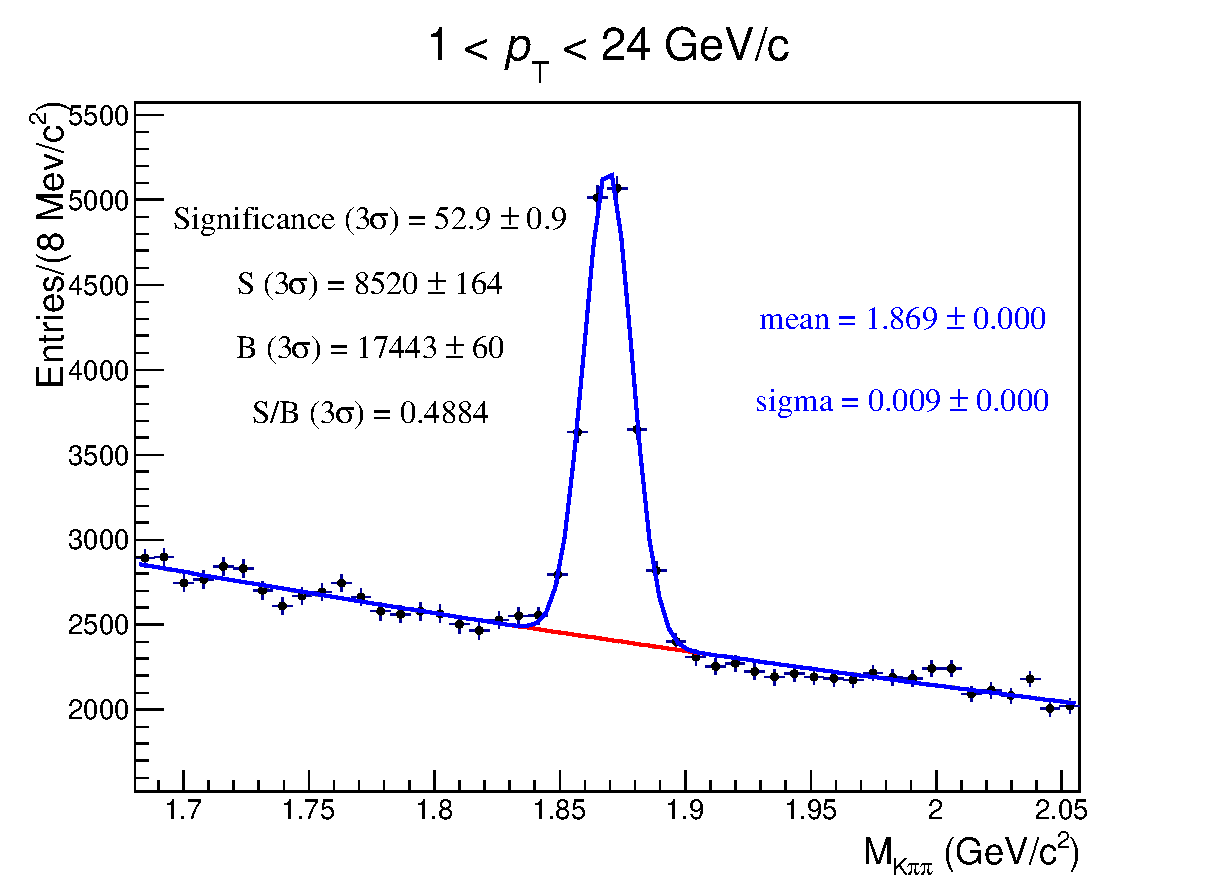
\includegraphics[scale=0.24]{MassFit_pt_1-24_fit.eps}}

\put(0,180){\captionsetup{labelformat=empty}
\begin{minipage}[t]{1.\linewidth}
Applicando tagli topologici per massimizzare il segnale su fondo $S/B$ e la significatività $sig = S/\sqrt{S+B}$, si prende soltanto una parte di essi
\end{minipage}}

\put(20,80){\includegraphics[scale=0.2]{DplusCand2.png}}

\put(102,110){
\begin{tikzpicture}[->]
\draw[draw=black,solid,line width=0.2mm] (1, 1) -- + (2.6, 0.);
\end{tikzpicture}}

\put(0,60){
\begin{minipage}[t]{0.5\linewidth}
\begin{center}
Il numero di $D^+$ ottenute dal fit di massa invariante (\textit{raw yield} $Y$) dipende perciò dalle efficienze di ricostruzione dei contributi prompt e feed-down
\end{center}
\end{minipage}}

\put(190,60){
\begin{minipage}[t]{0.35\linewidth}
\begin{block}{}
\setlength\abovedisplayskip{0pt}
\[\epsilon_{prompt}\textcolor{blue}{N_{prompt}}+\epsilon_{FD}\textcolor{red}{N_{FD}} = Y\]
\end{block}
\end{minipage}}

\end{picture}
\end{frame}

\begin{frame}
 \frametitle{Metodo della variazione dei tagli II}
\begin{picture}(320,250)

\put(0,230){
\begin{minipage}[t]{1.1\linewidth}
Se si considerano più set di tagli, si ottiene un sistema di equazioni
\end{minipage}}

\put(10,150){\includegraphics[scale=0.2]{DplusCand3.png}}

\put(170,220){
\begin{minipage}[t]{0.4\linewidth}
\begin{block}{}
\setlength\abovedisplayskip{0pt}
 \begin{equation*}
 \begin{cases}
 \epsilon_{prompt}^1N_{prompt}+\epsilon_{FD}^1N_{FD} = Y^1\\\\
 \textcolor{green}{\epsilon_{prompt}^2N_{prompt}+\epsilon_{FD}^2N_{FD} = Y^2}
 \end{cases}
 \end{equation*}
 \end{block}
\end{minipage}}

\put(90,185){
\begin{tikzpicture}[->]
\draw[draw=black,solid,line width=0.2mm] (1, 1) -- + (2.5, 0.5);
\end{tikzpicture}}

\put(87,173){
\begin{tikzpicture}[->]
\draw[draw=green,solid,line width=0.2mm] (1, 1) -- + (2.7, 0);
\end{tikzpicture}}

\put(0,130){
\begin{minipage}[t]{1.\linewidth}
\begin{center}
Se i set di tagli sono 2 allora il sistema è determinato, altrimenti è necessario trovare un metodo per valutare una soluzione approssimata 
\end{center}
\end{minipage}}

\put(10,110){
\begin{minipage}[t]{0.4\linewidth}
\setlength\abovedisplayskip{0pt}
\begin{block}{}
 \begin{equation*}
 \begin{cases}
 \epsilon_{prompt}^1N_{prompt}+\epsilon_{FD}^1N_{FD} = Y^1\\
 ...\\
 ...\\
 \epsilon_{prompt}^nN_{prompt}+\epsilon_{FD}^nN_{FD} = Y^n
 \end{cases}
 \end{equation*}
 \end{block}
\end{minipage}}

\put(180,85){
\begin{minipage}[t]{0.4\linewidth}
\begin{center}
$n$ set di tagli corrispondono a $n$ equazioni con soltanto\\ 2 variabili ($N_{prompt}$ e $N_{FD}$) \\$\Rightarrow$ il sistema è sovradeterminato
\end{center}
\end{minipage}}

\end{picture}
\end{frame}

\subsection{Metodo di Minimizzazione}
\begin{frame}
 \frametitle{Metodo di Minimizzazione}
% \framesubtitle{Method developed by Andrea Rossi and Felix Reidt for D$^0$ mesons}
\begin{picture}(320,250)

\put(10,230){
\begin{minipage}[t]{0.9\linewidth}
\begin{center}
Esprimendo il sistema di equazioni in notazione matriciale otteniamo\\
\begin{equation*}
\left(
\begin{array}{cc}
 \epsilon_{prompt}^1 & \epsilon_{FD}^1 \\
 .. & .. \\
 .. & .. \\
 \epsilon_{prompt}^n & \epsilon_{FD}^n \\ 
\end{array}
\right) \times
\left(
\begin{array}{c}
N_{prompt}\\
N_{FD}
\end{array}
\right)- 
\left(
\begin{array}{c}
Y^1\\
..\\
..\\
Y^n
\end{array}
\right) =
\left(
\begin{array}{c}
0\\
..\\
..\\
0
\end{array}
\right)
\end{equation*}

\vspace{0.4cm}
Sostituiamo il vettore nullo con un \textcolor{red}{vettore dei residui}\\
\begin{equation*}
\left(
\begin{array}{cc}
 \epsilon_{prompt}^1 & \epsilon_{FD}^1 \\
 .. & .. \\
 .. & .. \\
 \epsilon_{prompt}^n & \epsilon_{FD}^n \\ 
\end{array}
\right) \times
\left(
\begin{array}{c}
N_{prompt}\\
N_{FD}
\end{array}
\right)- 
\left(
\begin{array}{c}
Y^1\\
..\\
..\\
Y^n
\end{array}
\right) =
\textcolor{red}{\left(
\begin{array}{c}
\delta^1\\
..\\
..\\
\delta^n
\end{array}
\right)}
\end{equation*}

\vspace{0.4cm}
Per ottenere una soluzione approssimata è quindi necessario minimizzare il vettore dei residui
\end{center}
\end{minipage}}

\end{picture}
\end{frame}

\begin{frame}
\frametitle{Minimizzazione}
\begin{picture}(320,250)

\put(90,110){
\begin{minipage}[t]{0.5\linewidth}
\[
\sigma_i^2 = \sigma_{Y^i}^2+\sigma_{\epsilon_{prompt}^i}^2N_{prompt}^2+\sigma_{\epsilon_{FD}^i}^2N_{FD}^2
\]
\end{minipage}}

\put(110,225){
\begin{minipage}[t]{0.4\linewidth}
\begin{equation*}
C^{-1} =
\left(
\begin{array}{ccc}
1/\sigma_1^2 & & \\
 & \ddots &  \\
 & & 1/\sigma_n^2\\
\end{array}
\right)
\end{equation*}
\end{minipage}}

\put(60,60){
\begin{minipage}[t]{0.6\linewidth}
\begin{block}{}
\setlength\abovedisplayskip{0pt}
\[N = (\epsilon^TC^{-1}\epsilon)^{-1}(\epsilon^TC^{-1}Y) \quad Cov(N) = (\epsilon^TC^{-1}\epsilon)\]
\end{block}
\end{minipage}}

\put(-10,245){
\begin{minipage}[t]{1\linewidth}
\begin{itemize}
\item Definiamo il chi quadro come $\chi^2 = \delta^TC^{-1}\delta$, dove $C^{-1}$ è la matrice dei pesi

\vspace{2.6cm}
Le $\sigma_i$ sono valutate iterativamente 
\begin{itemize}
 \item nel primo step solo gli errori sui \textit{raw yield} sono considerati (siccome $N_{prompt}$ e $N_{FD}$ non sono conosciuti)
 \item dal secondo step vengono utilizzati nella propagazione dell'errore $N_{prompt}$ e $N_{FD}$ ottenuti dallo step precedente 
\end{itemize}

\vspace{1cm}
\item Il numero di $D^+$ prompt e feed-down è infine valutato minimizzando il $\chi^2$ ($\frac{d\chi^2}{dN_i} = 0$)
\end{itemize}
\end{minipage}}

\end{picture}
\end{frame}

\subsection{Metodo dell'incentro}
\begin{frame}
 \frametitle{Metodo dell'incentro}
%\framesubtitle{Method developed with Riccardo Russo}
 \begin{picture}(320,250)

\put(0,5){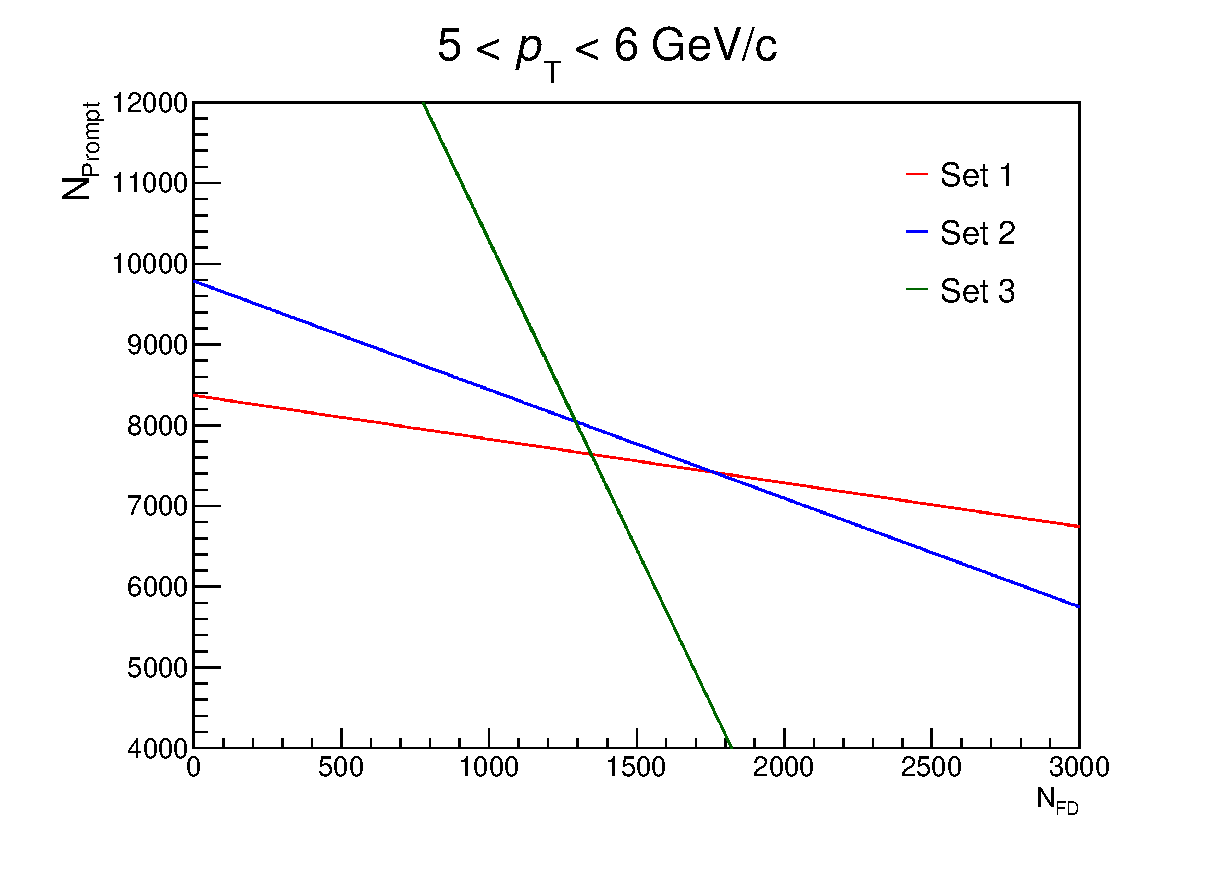
\includegraphics[scale=0.36]{Lines_5-6.eps}}

 \put(60,235){
\begin{minipage}[t]{0.6\linewidth}
\begin{block}{}
\setlength\abovedisplayskip{0pt}
\begin{equation*}
y = -\frac{\epsilon_{FD}^i}{\epsilon_{prompt}^i}x + \frac{Y^i}{\epsilon_{prompt}^i} \text{, \hspace{0.5cm}dove } 
\begin{cases}
 y = N_{prompt}\\
 x = N_{FD}
\end{cases}
\end{equation*}
\end{block}
\end{minipage}}

 \put(0,235){
\begin{minipage}[t]{1.\linewidth}
Ogni equazione del sistema descrive una retta 
\end{minipage}}

\put(0,175){
\begin{minipage}[t]{1.\linewidth}
Idealmente c'è soltanto un punto di intersezione tra tutte le rette, ma l'errore sull'estrazione del segnale e sulla determinazione dell'efficienza fa sì che ci siano $n$ intersezioni
\end{minipage}}

\put(85,68){
\begin{tikzpicture}
    \draw[draw=black,solid,line width=0.02cm] (0,0) ellipse (0.7cm and 0.4cm);
\end{tikzpicture}}

\put(215,65){\includegraphics[scale=0.28]{Incentre_def.png}}

\put(125,80){
\begin{tikzpicture}[->]
\draw[draw=black,solid,line width=0.2mm] (1, 1) -- + (3.7, 0.6);
\end{tikzpicture}}

\put(210,50){
 \begin{minipage}[t]{0.4\linewidth}
\begin{center}
 \textcolor{blue}{INCENTRO (I)}: punto di intersezione delle bisettrici
 \end{center}
 \end{minipage}}

\end{picture}
\end{frame}

\begin{frame}
 \frametitle{Errore sui parametri delle rette}
 \begin{picture}(320,250)

\put(0,230){
\begin{minipage}[t]{0.5\linewidth}
\begin{equation*}
N_{prompt} = -\frac{\epsilon_{FD}^i}{\epsilon_{prompt}^i}N_{FD} + \frac{Y^i}{\epsilon_{prompt}^i}
\end{equation*}
\end{minipage}}

\put(60,190){
\begin{tikzpicture}
    \draw[draw=blue,solid,line width=0.02cm] (0,0) ellipse (0.6cm and 0.8cm);
\end{tikzpicture}}

\put(40,178){
\begin{tikzpicture}[->]
\draw[draw=blue,solid,line width=0.2mm] (1, 1) -- + (-0.9, -0.6);
\end{tikzpicture}}

\put(118,190){
\begin{tikzpicture}
    \draw[draw=blue,solid,line width=0.02cm] (0,0) ellipse (0.6cm and 0.8cm);
\end{tikzpicture}}

\put(152,215){
\begin{tikzpicture}[->]
\draw[draw=blue,solid,line width=0.2mm] (1, 1) -- + (1., 0);
\end{tikzpicture}}

\put(120,20){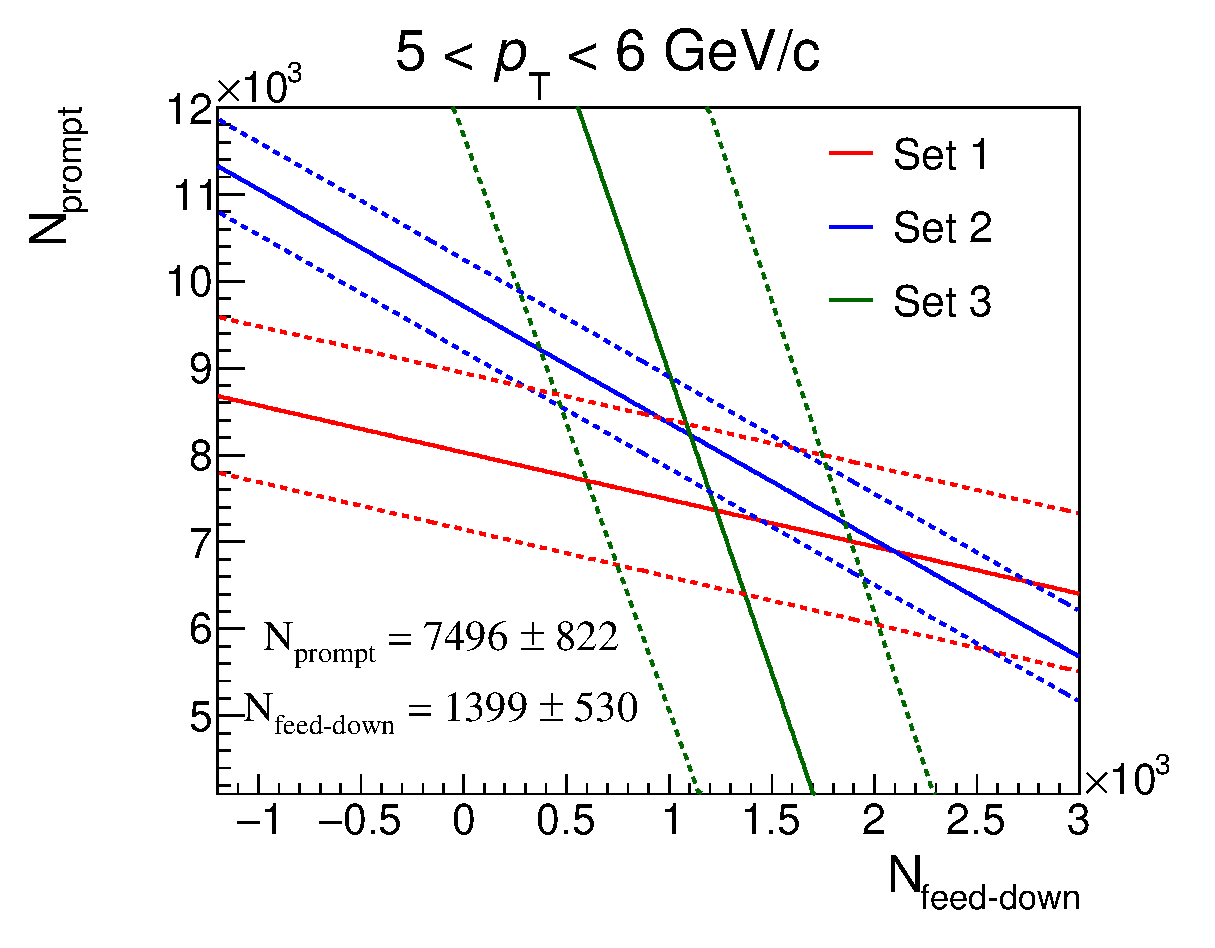
\includegraphics[scale=0.4]{LinesErr_5-6.eps}}

\put(0,165){
\begin{minipage}[t]{0.32\linewidth}
\begin{center}
L'errore sul coefficiente angolare è propagato dagli errori sulle efficienze
\end{center}
\end{minipage}}

\put(190,225){
\begin{minipage}[t]{0.35\linewidth}
\begin{center}
L'errore sul termine noto è dominato dall'incertezza sull'estrazione del segnale
\end{center}
\end{minipage}}

\put(0,100){
\begin{minipage}[t]{0.32\linewidth}
\begin{center}
 Il contributo maggiore all'errore deriva dall'incertezza sul \textit{raw yield}
\end{center}
\begin{equation*}
 \begin{cases}
 2\% \lesssim \Delta Y \lesssim 30\% \\
 1\% \lesssim \Delta\epsilon \lesssim 10\%
 \end{cases}
\end{equation*}
\end{minipage}}

 \end{picture}
\end{frame}
 
\begin{frame}
 \frametitle{Errore sulla determinazione dell'incentro}
 \begin{picture}(320,250)

 \put(200,105){\centering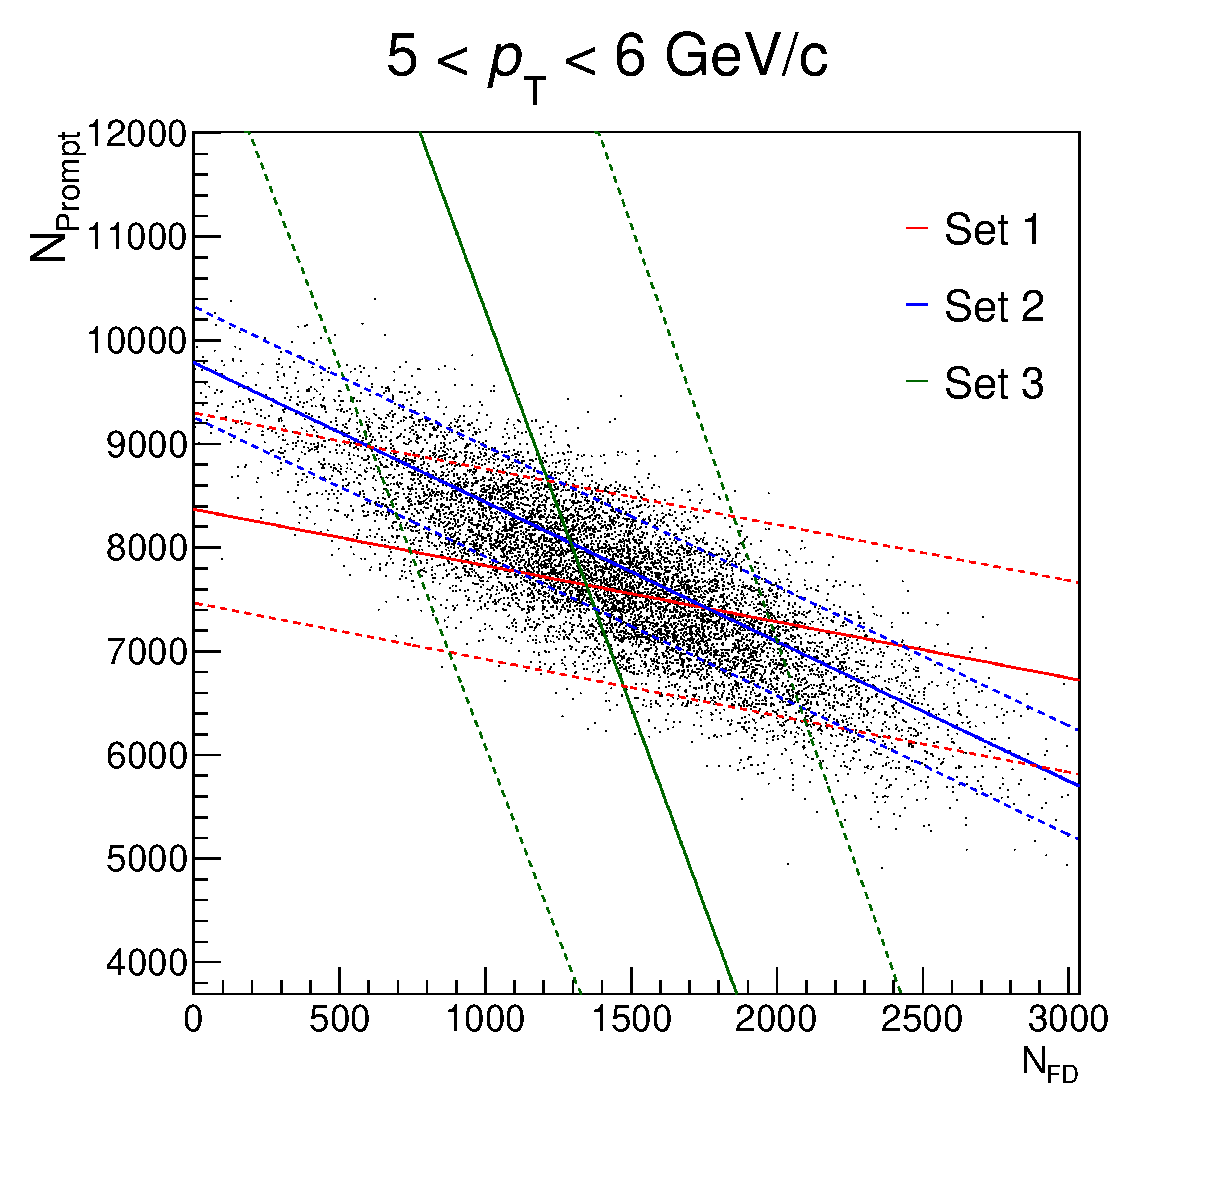
\includegraphics[scale = 0.26]{LinesDisp_5-6.eps}}

 \put(97,105){\centering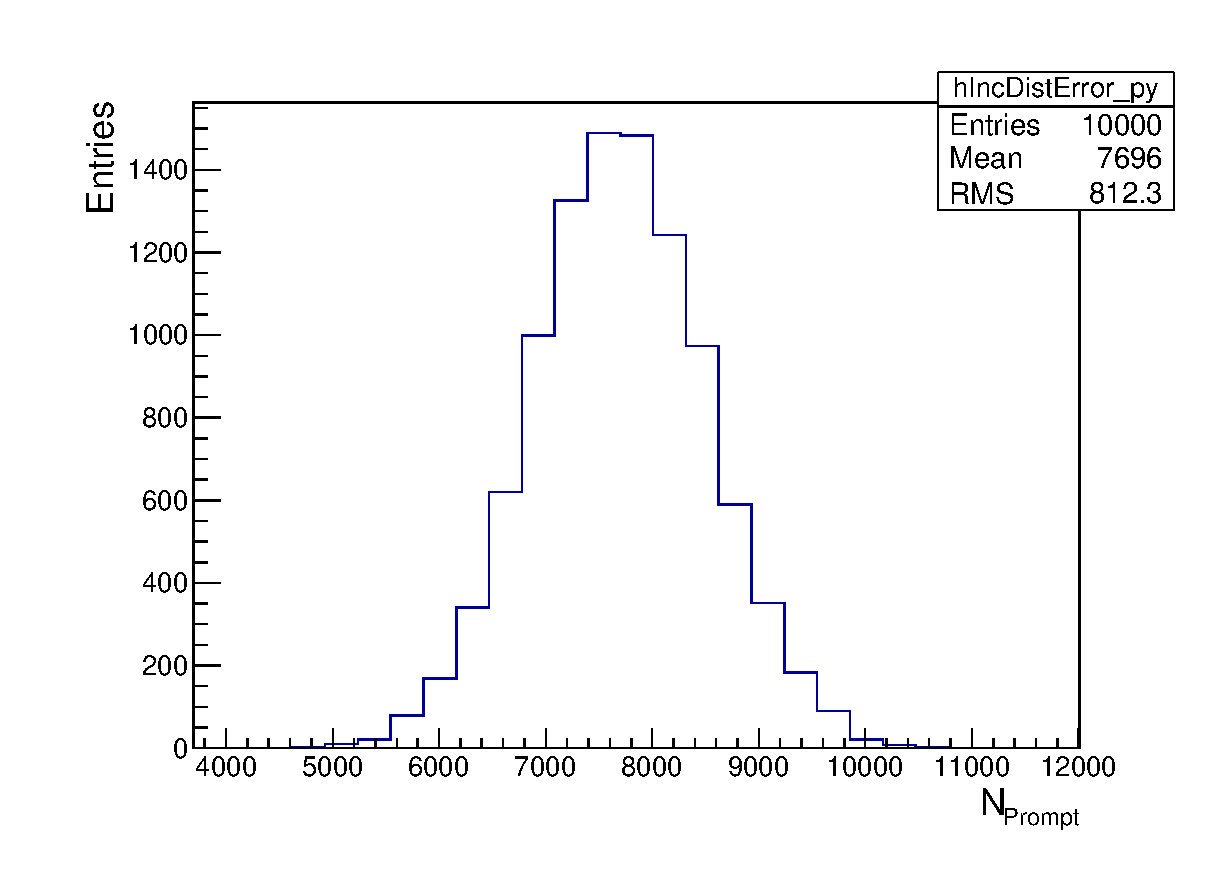
\includegraphics[scale=0.25, angle=90]{Nprompt_disp_5-6.eps}}

 \put(200,115){\reflectbox{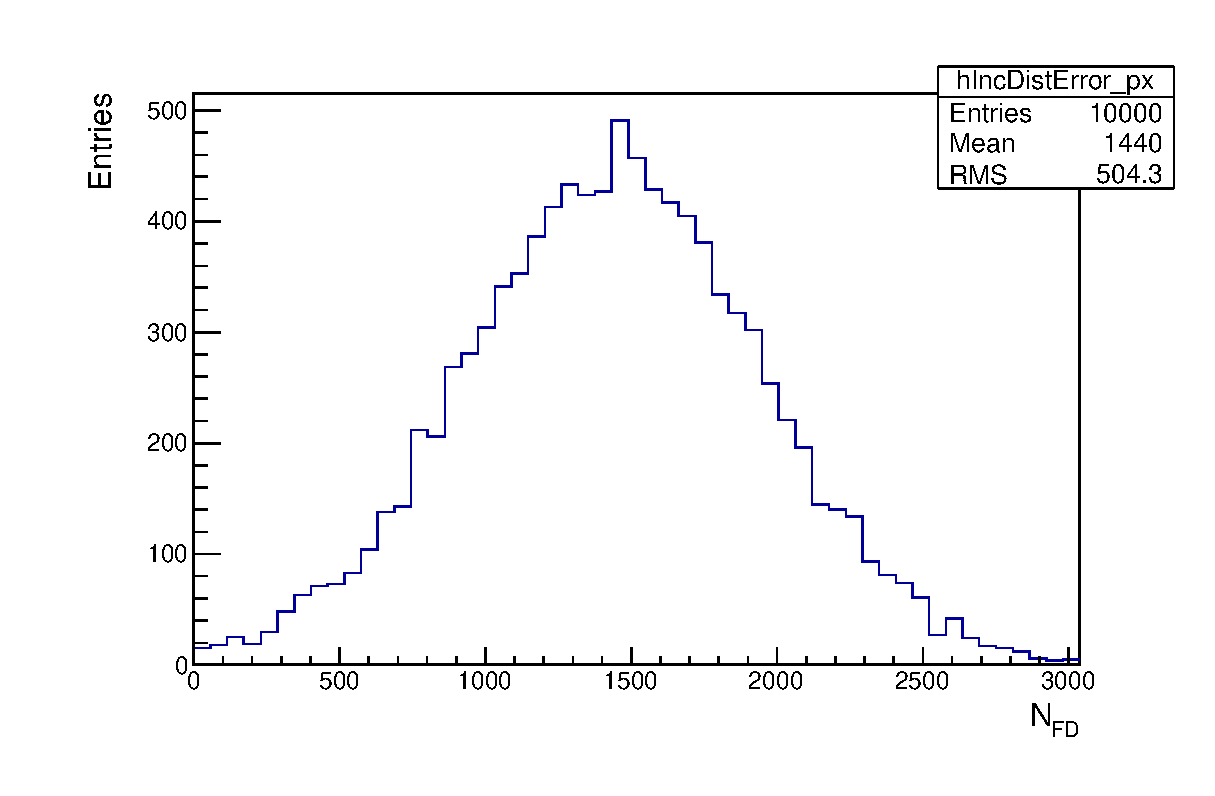
\includegraphics[scale=0.26, angle=180]{Nfeeddown_disp_5-6.eps}}}
 
\put(0,225){
\begin{minipage}[t]{0.25\linewidth}
L'errore è stato \\valutato con una \\\textcolor{blue}{simulazione MC}: 
\end{minipage}}

\put(-10,195){
\begin{minipage}[t]{0.3\linewidth}
\begin{itemize}
 \item i parametri vengono generati da una distribuzione gaussiana con valor medio il valore del parametro considerato e deviazione standard il suo errore
\end{itemize}
\end{minipage}}

\put(-10,93){
\begin{minipage}[t]{0.6\linewidth}
\begin{itemize}
 \item per ogni generazione random di tutti i parametri viene riempito un istogramma bidimensionale con le coordinate dell'incentro calcolato
\item l'errore su $N_{prompt}$ ed $N_{FD}$ è valutato come l'RMS delle distribuzioni proiettate sui rispettivi assi 
\end{itemize}
\end{minipage}}

\end{picture}
\end{frame}

\subsection{Set dei tagli}
\begin{frame}
 \frametitle{Strategia per la scelta dei tagli}
 \begin{picture}(320,250)

\put(10,235){
\begin{minipage}[t]{0.95\linewidth}
Per ottenere tre rette con coefficiente angolare più diverso possibile è necessario considerare dei set di tagli molto differenti tra loro
\end{minipage}}

\put(220,75){\includegraphics[scale=0.18]{vars.png}}
\put(0,15){\includegraphics[scale=0.2]{d0d0exp.png}}

 \put(7,225){
\begin{minipage}[t]{0.95\linewidth}
\begin{block}{}
\setlength\abovedisplayskip{0pt}
\begin{itemize}
 \item 1$^o$ set: massimizzazione dell'efficienza di selezione delle $D^+$ prompt
 \item 2$^o$ set: massimizzazione della significatività
 \item 3$^o$ set: massimizzazione dell'efficienza di selezione delle $D^+$ feed-down
\end{itemize}
\end{block}
\end{minipage}}

\put(0,155){
\begin{minipage}[t]{0.7\linewidth}
Le variabili scelte devono perciò poter separare \\i contributi di prompt e feed-down:
\begin{enumerate}
 \item coseno dell'angolo di \textit{pointing} nel piano $XY$ ($cos(\theta_P^{XY})$)
 \item lunghezza di decadimento nel piano $XY$ ($L_{XY}$)
 \item lunghezza di decadimento nel piano $XY$ \\normalizzata al proprio errore ($norm\text{ }L_{XY}$)
\end{enumerate}
\end{minipage}}

\put(135,75){
\begin{minipage}[t]{0.63\linewidth}
\begin{enumerate}
\addtocounter{enumi}{3}
 \item Massimo residuo del parametro di impatto delle tracce delle particelle figlie ($norm\text{ }max\text{ }d_0-d_0exp$)
\[max\text{ }n\sigma_{res} = max\text{ }\frac{d_0^{exp}-d_0^{reco}}{\sqrt{\sigma^2(d_0^{reco})+\sigma^2(d_0^{exp})}}\]
\end{enumerate}
\end{minipage}}

\put(80,35){
\begin{minipage}[t]{0.2\linewidth}
\[d_0^{exp} \approx L_{XY}\sin(\theta_{XY}^{tr})\]
\end{minipage}}

\end{picture}
\end{frame}

\begin{frame}
\frametitle{Distribuzioni MC delle variabili per $D^+$ prompt e feed-down}
\begin{picture}(320,250)

\put(20,130){\includegraphics[scale=0.24]{Dist_cxy_5-6.eps}}
\put(20,13){\includegraphics[scale=0.24]{Dist_NLxy_5-6.eps}}
\put(190,130){\includegraphics[scale=0.24]{Dist_Lxy_5-6.eps}}
\put(190,13){\includegraphics[scale=0.24]{Dist_d0d0exp_5-6.eps}}

\put(0,240){
\begin{minipage}[t]{0.3\linewidth}
\begin{enumerate}
\addtocounter{enumi}{0}
\item$\cos(\theta_P^{XY})$
\end{enumerate}
\end{minipage}}

\put(170,240){
\begin{minipage}[t]{0.3\linewidth}
\begin{enumerate}
\addtocounter{enumi}{1}
\item$L_{XY}$
\end{enumerate}
\end{minipage}}

\put(0,130){
\begin{minipage}[t]{0.3\linewidth}
\begin{enumerate}
\addtocounter{enumi}{2}
\item$Norm\text{ }L_{XY}$
\end{enumerate}
\end{minipage}}

\put(170,130){
\begin{minipage}[t]{0.3\linewidth}
\begin{enumerate}
\addtocounter{enumi}{3}
\item$Norm\text{ }max\text{ }d_0-d_0exp$
\end{enumerate}
\end{minipage}}

\end{picture}
\end{frame}

\subsection{Efficienze}
\begin{frame}
\frametitle{Efficienze - Set 1}
\begin{picture}(320,250)

\put(10,100){\includegraphics[scale=0.36]{Eff_Set1.eps}}

\put(210,205){
\begin{minipage}[t]{0.35\linewidth}
\begin{center}
Il primo set di tagli è stato ottimizzato per massimizzare l'efficienza delle $D^+$ prompt rispetto alle $D^+$ feed-down 
\end{center}
\[ 1.5 \lesssim \frac{\epsilon_{prompt}}{\epsilon_{FD}} \lesssim 2 \]
\end{minipage}}

\put(25,60){\captionsetup{labelformat=empty}
\begin{minipage}[t]{0.36\linewidth}
\renewcommand\arraystretch{1.4} 
  \begin{tabular}{c|c|c|c|c}
    $p_T (GeV/c)$ & $\cos(\theta_P^{XY})$ & $L_{XY} (cm)$ & $Norm\text{ }L_{XY}$ & $Norm\text{ }max\text{ }d_0-d_0exp$ \\
    \hline
    $2-4$ &$[0.998,1]$ & $[0.02,0.14]$ & $[7,12]$ & $[-1.5,1.5]$ \\
    \hline
    $4-8$ &$[0.998,1]$ & $[0.02,0.15]$ & $[4,16]$ & $[-1.5,1.5]$ \\
    \hline
    $8-12$ &$[0.998,1]$ & $[0.04,0.15]$ & $[4,16]$ & $[-1.5,1.5]$ \\
     \hline
    $12-16$ &$[0.998,1]$ & $[0.04,0.25]$ & $[4,22]$ & $[-2.0,2.0]$ \\
    \end{tabular}
\end{minipage}}

\end{picture}
\end{frame}

\begin{frame}
\frametitle{Efficienze - Set 2}
\begin{picture}(320,250)

\put(10,95){\includegraphics[scale=0.36]{Eff_Set2.eps}}

\put(210,200){
\begin{minipage}[t]{0.35\linewidth}
\begin{center}
Il secondo set di tagli è stato ottimizzato per massimizzare il segnale estratto dai fit degli spettri di massa invariante  
\end{center}
\[ 1.2 \lesssim \frac{\epsilon_{FD}}{\epsilon_{prompt}} \lesssim 1.5 \]
\end{minipage}}

\put(25,60){\captionsetup{labelformat=empty}
\begin{minipage}[t]{0.36\linewidth}
\renewcommand\arraystretch{1.4} 
  \begin{tabular}{c|c|c|c|c}
    $p_T (GeV/c)$ & $\cos(\theta_P^{XY})$ & $L_{XY} (cm)$ & $Norm\text{ }L_{XY}$ & $Norm\text{ }max\text{ }d_0-d_0exp$ \\
    \hline
    $2-12$ &$[0.990,1]$ & $>0.05$ & $>9$ & $/$ \\
    \hline
    $12-16$ &$[0.990,1]$ & $>0.10$ & $>6$ & $/$ \\
    \end{tabular}
\end{minipage}}

\end{picture}
\end{frame}

\begin{frame}
\frametitle{Efficienze - Set 3}
\begin{picture}(320,250)

\put(10,100){\includegraphics[scale=0.36]{Eff_Set3.eps}}

\put(210,205){
\begin{minipage}[t]{0.35\linewidth}
\begin{center}
Il terzo set di tagli è stato ottimizzato per massimizzare l'efficienza delle $D^+$ feed-down rispetto alle $D^+$ prompt 
\end{center}
\[ 4 \lesssim \frac{\epsilon_{FD}}{\epsilon_{prompt}} \lesssim 10 \]
\end{minipage}}

\put(25,60){\captionsetup{labelformat=empty}
\begin{minipage}[t]{0.36\linewidth}
\renewcommand\arraystretch{1.4} 
  \begin{tabular}{c|c|c|c|c}
    $p_T (GeV/c)$ & $\cos(\theta_P^{XY})$ & $L_{XY} (cm)$ & $Norm\text{ }L_{XY}$ & $Norm\text{ }max\text{ }d_0-d_0exp$ \\
    \hline
    $2-4$ &$[0.990,1]$ & $>0.08$ & $>9$ & $<-2$ \\
    \hline
    $4-6$ &$[0.990,1]$ & $>0.12$ & $>12$ & $<-2$ \\
    \hline
    $6-12$ &$[0.990,1]$ & $>0.20$ & $>16$ & $<-2$ \\
    \hline
    $12-16$ &$[0.990,1]$ & $>0.20$ & $>22$ & $<-1.5$ \\
    \end{tabular}
\end{minipage}}

\end{picture}
\end{frame}

\subsection{Estrazione del segnale}
\begin{frame}
\frametitle{Estrazione del segnale}
\begin{picture}(320,250)

\put(20,140){\includegraphics[scale=0.25]{Fitter_5_fit_set1.eps}}
\put(180,140){\includegraphics[scale=0.25]{Fitter_5_fit_set2.eps}}
\put(20,25){\includegraphics[scale=0.25]{Fitter_5_fit_set3.eps}}

\put(185,110){
\begin{minipage}[t]{0.4\linewidth}
\begin{center}
Per i set di tagli 1 e 3 la selezione di uno solo dei due contributi (prompt o feed-down) determina una significatività più bassa nell'estrazione del segnale ($sig \approx 5$) rispetto al set centrale ($sig \approx 15-20$)    
\end{center}
\end{minipage}}

\end{picture}
\end{frame}

\subsection{Risultato}
\begin{frame}
\frametitle{Sezione d'urto $D^+$ prompt}
\begin{picture}(320,250)

\put(-5,5){\includegraphics[scale=0.37]{CrossSectionPromptpPb.eps}}
\put(195,30){\includegraphics[scale=0.28]{RatioPublishedPromptpPb.eps}}

\put(210,220){
\begin{minipage}[t]{0.35\linewidth}
\begin{center}
La sezione d'urto dei mesoni $D^+$ prompt ottenuta con il metodo della variazione dei tagli risulta compatibile con quella pubblicata, pur rimanendo sistematicamente inferiore 
\end{center}
\end{minipage}}

\put(35,245){
\begin{minipage}[t]{0.4\linewidth}
\begin{block}{}
\setlength\abovedisplayskip{0pt}
\[ \frac{d\sigma_{prompt}^{D^+}}{dp_T} = \frac{1}{2} \frac{\sigma_{pPb}}{Acc\cdot N_{ev}\cdot BR}\frac{N_{prompt}}{\Delta p_T}\]
\end{block}
\end{minipage}}

\end{picture}
\end{frame}

\begin{frame}
\frametitle{Sezione d'urto $D^+$ feed-down}
\begin{picture}(320,250)

\put(-5,5){\includegraphics[scale=0.37]{CrossSectionFDpPb.eps}}  
\put(195,20){\includegraphics[scale=0.28]{RatioMethodsFDpPb.eps}}  

\put(210,230){
\begin{minipage}[t]{0.36\linewidth}
\begin{center}
La sezione d'urto dei mesoni $D^+$ feed-down ottenuta con il metodo della variazione dei tagli risulta compatibile con la predizione di \textit{FONLL} riscalata per il numero di nucleoni del $Pb$ ad alto momento trasverso ($p_T > 6 \text{ } GeV/c$), mentre sembra essere maggiore a basso $p_T$  
\end{center}
\end{minipage}}

\put(35,245){
\begin{minipage}[t]{0.4\linewidth}
\begin{block}{}
\setlength\abovedisplayskip{0pt}
\[ \frac{d\sigma_{FD}^{D^+}}{dp_T} = \frac{1}{2} \frac{\sigma_{pPb}}{Acc\cdot N_{ev}\cdot BR}\frac{N_{FD}}{\Delta p_T}\]
\end{block}
\end{minipage}}

\end{picture}
\end{frame}

\section{Confronto}
\begin{frame}
\frametitle{Confronto dei metodi \textit{data-driven} con il risultato pubblicato}
\begin{picture}(320,250)

\put(210,210){
\begin{minipage}[t]{0.36\linewidth}
\begin{center}
La sezione d'urto dei mesoni $D^+$ prompt ottenuta con i metodi \textit{data-driven} risulta in buon accordo con il risultato pubblicato, in cui sono stati utilizzati i metodi \textit{theory-driven} 
\end{center}
\end{minipage}}

\put(-5,40){\includegraphics[scale=0.37]{CrossSecComp.eps}}  
\put(195,20){\includegraphics[scale=0.28]{CrossSecRatios.eps}}  

\put(0,235){
\begin{minipage}[t]{1.\linewidth}
\begin{center}
\end{center}
\end{minipage}}

\end{picture}
\end{frame}

\section{Attività future}
\begin{frame}
\frametitle{Attività future}
\begin{picture}(320,250)

\put(0,225){
\begin{minipage}[t]{1.\linewidth}
Il mio progetto di tesi prevede ancora:
\begin{enumerate}
%\item conclusione della valutazione degli errori sistematici per il metodo di fit del parametro di impatto 
 \item valutazione degli errori sistematici per il metodo della variazione dei tagli
\begin{itemize}
 \item incertezza dovuta alla scelta dei set di tagli
 \item incertezza nell'estrazione del segnale (raw yield)
 \item incertezza sull'efficienza 
 \end{itemize}
% \item (inizio) di analisi dei dati $Pb-Pb$ raccolti durante il RUN II di LHC all'esperimento ALICE
 \item periodo di lavoro al centro di ricerca GSI (Darmstadt)
 \end{enumerate}
\end{minipage}}

\put(100,60){
\begin{minipage}[t]{1.\linewidth}
\Huge{\textcolor{blue}{GRAZIE PER L'ATTENZIONE!}}
\end{minipage}}

\end{picture}
\end{frame}

\section{Backup}
\begin{frame}
\frametitle{}
\begin{picture}(320,250)

\put(70,180){
\begin{minipage}[t]{0.55\linewidth}
\begin{block}{}
\begin{center}
\fontsize{1.5cm}{1.75cm}\selectfont{\textcolor{blue}{BACKUP}}
\end{center}
\end{block}
\end{minipage}}

\end{picture}
\end{frame}

\subsection{Prefit delle distribuzioni MC}
\begin{frame}
\frametitle{Prefit delle distribuzioni MC delle $D^+$ prompt}
\begin{picture}(320,250)
\put(10,170){\includegraphics[scale=0.18]{ImpParPrompt_2-3.eps}}  
\put(120,170){\includegraphics[scale=0.18]{ImpParPrompt_3-4.eps}}  
\put(230,170){\includegraphics[scale=0.18]{ImpParPrompt_4-5.eps}}  
\put(10,90){\includegraphics[scale=0.18]{ImpParPrompt_5-6.eps}}  
\put(120,90){\includegraphics[scale=0.18]{ImpParPrompt_6-8.eps}}  
\put(230,90){\includegraphics[scale=0.18]{ImpParPrompt_8-12.eps}}  
\put(120,10){\includegraphics[scale=0.18]{ImpParPrompt_12-16.eps}}  
\end{picture}
\end{frame}

\begin{frame}
\frametitle{Prefit delle distribuzioni MC delle $D^+$ feed-down I}
\begin{picture}(320,250)
\put(10,170){\includegraphics[scale=0.18]{ImpParTrueFD_2-3.eps}}  
\put(120,170){\includegraphics[scale=0.18]{ImpParTrueFD_3-4.eps}}  
\put(230,170){\includegraphics[scale=0.18]{ImpParTrueFD_4-5.eps}}  
\put(10,90){\includegraphics[scale=0.18]{ImpParTrueFD_5-6.eps}}  
\put(120,90){\includegraphics[scale=0.18]{ImpParTrueFD_6-8.eps}}  
\put(230,90){\includegraphics[scale=0.18]{ImpParTrueFD_8-12.eps}}  
\put(120,10){\includegraphics[scale=0.18]{ImpParTrueFD_12-16.eps}}  
\end{picture}
\end{frame}

\begin{frame}
\frametitle{Prefit delle distribuzioni MC delle $D^+$ feed-down II}
\begin{picture}(320,250)
\put(10,170){\includegraphics[scale=0.18]{ImpParRecoFD_2-3.eps}}  
\put(120,170){\includegraphics[scale=0.18]{ImpParRecoFD_3-4.eps}}  
\put(230,170){\includegraphics[scale=0.18]{ImpParRecoFD_4-5.eps}}  
\put(10,90){\includegraphics[scale=0.18]{ImpParRecoFD_5-6.eps}}  
\put(120,90){\includegraphics[scale=0.18]{ImpParRecoFD_6-8.eps}}  
\put(230,90){\includegraphics[scale=0.18]{ImpParRecoFD_8-12.eps}}  
\put(120,10){\includegraphics[scale=0.18]{ImpParRecoFD_12-16.eps}}  
\end{picture}
\end{frame}

\subsection{Prefit delle distribuzioni delle sidebands}
\begin{frame}
\frametitle{Prefit delle distribuzioni delle sidebands}
\begin{picture}(320,250)
\put(10,170){\includegraphics[scale=0.18]{ImpParBkg_2-3.eps}}  
\put(120,170){\includegraphics[scale=0.18]{ImpParBkg_3-4.eps}}  
\put(230,170){\includegraphics[scale=0.18]{ImpParBkg_4-5.eps}}  
\put(10,90){\includegraphics[scale=0.18]{ImpParBkg_5-6.eps}}  
\put(120,90){\includegraphics[scale=0.18]{ImpParBkg_6-8.eps}}  
\put(230,90){\includegraphics[scale=0.18]{ImpParBkg_8-12.eps}}  
\put(120,10){\includegraphics[scale=0.18]{ImpParBkg_12-16.eps}}  
\end{picture}
\end{frame}

\subsection{Fit delle distribuzioni del parametro di impatto}
\begin{frame}
\frametitle{Fit delle distribuzioni del parametro di impatto}
\begin{picture}(320,250)
\put(10,170){\includegraphics[scale=0.18]{FitUnbinned_2-3_bkg_plot.eps}}  
\put(120,170){\includegraphics[scale=0.18]{FitUnbinned_3-4_bkg_plot.eps}}  
\put(230,170){\includegraphics[scale=0.18]{FitUnbinned_4-5_bkg_plot.eps}}  
\put(10,90){\includegraphics[scale=0.18]{FitUnbinned_5-6_bkg_plot.eps}}  
\put(120,90){\includegraphics[scale=0.18]{FitUnbinned_6-8_bkg_plot.eps}}  
\put(230,90){\includegraphics[scale=0.18]{FitUnbinned_8-12_bkg_plot.eps}}  
\put(120,10){\includegraphics[scale=0.18]{FitUnbinned_12-16_bkg_plot.eps}}  
\end{picture}
\end{frame}

\begin{frame}
\frametitle{Distribuzione del parametro di impatto del fondo - dipendenza da $M$}
\begin{picture}(320,250)

\put(0,230){\captionsetup{labelformat=empty}
\begin{minipage}[t]{1.\linewidth}
\begin{center}
Per verificare che la distribuzione delle \textit{sidebands} non dipende dal range di massa a lato del picco si possono effettuare i prefit in diversi intervalli di massa invariante
\end{center}
\end{minipage}}

\put(15,30){\includegraphics[scale=0.45]{SB_pars_pT_2-3.eps}}

\put(185,105){\captionsetup{labelformat=empty}
\begin{minipage}[t]{0.44\linewidth}
\begin{center}
I parametri del fit non mostrano una marcata dipendenza dall'intervallo di massa considerato, anche se sembra esserci una differenza tra la regione a destra e sinistra del picco \\
$\Rightarrow$ di questo effetto si è tenuto conto nella valutazione degli errori sistematici
\end{center}
\end{minipage}}

\end{picture} 
\end{frame}

\begin{frame}
\frametitle{Distribuzione del parametro di impatto del fondo - funzione di fit delle \textit{sidebands}}
\begin{picture}(320,250)

\put(15,130){\includegraphics[scale=0.25]{ImpParBkg_4-5.eps}}
\put(180,130){\includegraphics[scale=0.25]{ImpParBkg_4-5_asymm.eps}}
\put(15,25){\includegraphics[scale=0.25]{ImpParBkg_12-16.eps}}
\put(180,25){\includegraphics[scale=0.25]{ImpParBkg_12-16_asymm.eps}}

\put(40,235){\captionsetup{labelformat=empty}
\begin{minipage}[t]{1.\linewidth}
\textcolor{blue}{Funzione simmetrica \hspace{2.7cm} Funzione asimmetrica}
\end{minipage}}

\end{picture} 
\end{frame}

\subsection{Metodo dell'incentro (variazione dei tagli)}
\begin{frame}
\frametitle{Intersezioni tra le rette - metodo dell'incentro}
\begin{picture}(320,250)
\put(10,165){\includegraphics[scale=0.15]{LinesDisp_2-3.eps}}  
\put(120,165){\includegraphics[scale=0.15]{LinesDisp_3-4.eps}}  
\put(230,165){\includegraphics[scale=0.15]{LinesDisp_4-5.eps}}  
\put(10,85){\includegraphics[scale=0.15]{LinesDisp_5-6.eps}}  
\put(120,85){\includegraphics[scale=0.15]{LinesDisp_6-8.eps}}  
\put(230,85){\includegraphics[scale=0.15]{LinesDisp_8-12.eps}}  
\put(120,5){\includegraphics[scale=0.15]{LinesDisp_12-16.eps}}  
\end{picture}
\end{frame}

\end{document}